\documentclass[12pt,a4paper]{report}
\usepackage{fontspec}
\usepackage{setspace}
\usepackage{needspace}
\setmainfont{Times New Roman}
\usepackage[utf8]{inputenc}
\usepackage[margin=2.5cm]{geometry}
\usepackage{graphicx}
\usepackage{fancyhdr}
\usepackage{setspace}
\usepackage{framed}
\usepackage{titlesec}
\usepackage{titling}
\usepackage{lipsum}
\usepackage{listings}
\usepackage{hyperref}
\usepackage{color}
\usepackage{indentfirst} 
\setlength{\parindent}{15pt}
\usepackage{subcaption}
\usepackage[utf8]{inputenc}
\usepackage{graphicx}
\usepackage{tcolorbox}
\usepackage{xcolor}
\usepackage{geometry}
\usepackage{float}
\usepackage{titlesec}
\titleformat{\subsection}
  {\normalfont\normalsize\bfseries}{\thesubsection}{1em}{}
\titlespacing*{\subsection}
  {0pt}{3.25ex plus 1ex minus .2ex}{1.5ex plus .2ex}
\usepackage{lipsum}
\usepackage{hyperref}
\usepackage[top=2.5cm, bottom=2.5cm, left=3cm, right=2.5cm]
%\renewcommand{\contentsname}{}
%\renewcommand{\refname}{}
%\renewcommand{\bibname}{}

\definecolor{codegreen}{rgb}{0,0.6,0}
\definecolor{codegray}{rgb}{0.5,0.5,0.5}
\definecolor{codepurple}{rgb}{0.58,0,0.82}
\definecolor{backcolour}{rgb}{0.95,0.95,0.92}

\lstdefinestyle{mystyle}{
    backgroundcolor=\color{backcolour},   
    commentstyle=\color{codegreen},
    keywordstyle=\color{magenta},
    numberstyle=\tiny\color{codegray},
    stringstyle=\color{codepurple},
    basicstyle=\ttfamily\footnotesize,
    breakatwhitespace=false,         
    breaklines=true,                 
    captionpos=b,                    
    keepspaces=true,                 
    numbers=left,                    
    numbersep=5pt,                  
    showspaces=false,                
    showstringspaces=false,
    showtabs=false,                  
    tabsize=2
}
\pagestyle{empty}
\definecolor{mintgreen}{HTML}{9DEBD1}

\hypersetup{
    colorlinks=false,
    allbordercolors=mintgreen
}

\onehalfspacing
\begin{document}
\begin{center}

    
\includegraphics[width=5cm]{images/morsli/logo-univ-.png} \\[0.5cm]

    \color{mintgreen}
    \rule{\linewidth}{2pt}
    
    \color{black}
    \vspace{0.3cm}
    \textbf{\large People's Democratic Republic of Algeria} \\
    \textbf{Ministry of Higher Education and Scientific Research} \\
    \textbf{University of Ahmed Draia – Adrar} \\
    \textbf{Faculty of Science and Technology} \\
    \textbf{Department of Mathematics and Computer Science} \\

    \vspace{0.3cm}
    \textit{A dissertation submitted in partial fulfillment of the requirements for the} \\
    \textbf{Bachelor's degree in Science and Technology} \\
    Major: \textbf{Computer Science} \\

    \vspace{0.5cm}
    {\color{mintgreen} \rule{0.8\linewidth}{1.5pt} }

    \begin{tcolorbox}[colback=mintgreen!20, colframe=mintgreen!80!black, width=0.9\linewidth, boxrule=1pt, arc=5pt, auto outer arc]
        \centering
        \Large \textbf{Mobile Application for Student Attendance Tracking Using QR Code}
    \end{tcolorbox}

    \vspace{1cm}
    \textbf{Prepared by:} \\[0.2cm]
    ZAAF Hachem Rachid \\
    KENADIL Riham \\
    MORSLI Amira Djihane \\

    \vspace{1cm}
    \textbf{Under the supervision of:} \\[0.2cm]
    DR. LMTENECHE Sami \\


    
    \vspace{1cm}
    \textbf{Jury Committee:} \\[0.2cm]
    DR.  OUEHAB Abdel Ouehab : President \\
    DR. DEMRI Mohammed : Examiner \\

    \vfill
    \textbf{Academic Year: 2024–2025}

\end{center}

\newpage
\newenvironment{Summary}{
    \newpage
    \phantomsection
    \addcontentsline{toc}{chapter}{Summary}
    \begin{center}
        {\color{mintgreen} \rule{\textwidth}{2pt} }\\[0.3cm]
        {\Large \textbf{Summary}}\\[0.3cm]
        {\color{mintgreen} \rule{0.8\textwidth}{1.5pt} }
    \end{center}
    \vspace{0.5cm}
    \noindent
}{
    \vspace{0.5cm}
    \begin{center}
        {\color{mintgreen} \rule{0.8\textwidth}{1.5pt} }\\[0.3cm]
        {\color{mintgreen} \rule{\textwidth}{2pt} }
    \end{center}
}


\begin{Summary}
The implementation of a QR-based attendance tracking application within academic institutions has emerged as a critical necessity for optimizing educational administrative workflows. This QR Code attendence application delivers robust and comprehensive solutions for faculty and administration staff, permitting seamless real-time presence verification without reliance on conventional paper documentation methods.

Additionally, these systems provide instructors with instant access to precise and current attendance data and student participation metrics. The successful deployment of efficient attendance tracking mechanisms necessitates integration of contemporary technological components, including secure centralized data repositories, intuitive mobile interfaces, and reliable QR code functionality, ensuring reliability, operational streamlining, and prevention of fraudulent entries.

This initiative focuses on developing and deploying a sophisticated mobile platform that resolves traditional attendance monitoring limitations, enabling student participation verification through straightforward QR code scanning procedures. The application incorporates sophisticated analytical tools customized to specific academic departmental requirements, resulting in significant improvements to instructional efficiency and reduction of administrative overhead. Additionally, it strengthens educational outcomes and encourages student accountability by establishing transparent mechanisms for monitoring classroom engagement and participation rates.
\end{Summary}


\newpage
\newenvironment{ملخص}{
    \newpage
    \phantomsection
    \addcontentsline{toc}{chapter}{ملخص}
    \begin{center}
        {\color{mintgreen} \rule{\textwidth}{2pt} }\\[0.3cm]
        {\Large \textbf{الملخص}}\\[0.3cm]
        {\color{mintgreen} \rule{0.8\textwidth}{1.5pt} }
    \end{center}
    \vspace{0.5cm}
    \noindent
}{
    \vspace{0.5cm}
    \begin{center}
        {\color{mintgreen} \rule{0.8\textwidth}{1.5pt} }\\[0.3cm]
        {\color{mintgreen} \rule{\textwidth}{2pt} }
    \end{center}
}

\begin{ملخص}
أصبح تنفيذ تطبيق لتتبع الحضور باستخدام رمز الاستجابة السريعة (QR) داخل المؤسسات الأكاديمية ضرورة ملحة لتحسين سير العمل الإداري في العملية التعليمية. يوفر هذا التطبيق حلاً شاملاً وفعالاً للأساتذة، مما يسمح بالتحقق الفوري من الحضور دون الاعتماد على الطرق التقليدية الورقية.
تيح هذا النظام للمدرسين الوصول الفوري إلى بيانات دقيقة ومحدّثة حول الحضور ومعدلات مشاركة الطلبة، مما يسهم في تحسين تنظيم العملية التعليمية واتخاذ القرارات بشكل أسرع وأكثر فعالية. ويتطلب تنفيذ نظام تتبع حضور ناجح دمج تقنيات حديثة، مثل قواعد البيانات المركزية الآمنة، وواجهات الاستخدام السهلة على الهواتف الذكية، ووظائف قراءة رموز QR الموثوقة، لضمان الكفاءة، والسرعة، والحد من محاولات التلاعب.

يركّز هذا المشروع على تطوير ونشر منصة محمولة متقدمة تعالج القيود التقليدية لأنظمة تتبع الحضور، من خلال تمكين الطلبة من تأكيد حضورهم ببساطة عبر مسح رمز الاستجابة السريعة. كما يدمج التطبيق أدوات تحليل ذكية تلبي احتياجات الأقسام الأكاديمية المختلفة، مما يؤدي إلى تحسين كفاءة التدريس وتقليل الأعباء الإدارية. إضافة إلى ذلك، يساهم في تحسين النتائج التعليمية وتعزيز انضباط الطلبة من خلال توفير آليات شفافة لرصد المشاركة والتفاعل داخل الصف.
\end{ملخص}




\newpage
\newenvironment{Acknowledgment}{
    \newpage
    \phantomsection
    \addcontentsline{toc}{chapter}{Acknowledgment}
    \begin{center}
        {\color{mintgreen} \rule{\textwidth}{2pt} }\\[0.3cm]
        {\Large \textbf{Acknowledgment}}\\[0.3cm]
        {\color{mintgreen} \rule{0.8\textwidth}{1.5pt} }
    \end{center}
    \vspace{0.5cm}
    \noindent
}{
    \vspace{0.5cm}
    \begin{center}
        {\color{mintgreen} \rule{0.8\textwidth}{1.5pt} }\\[0.3cm]
        {\color{mintgreen} \rule{\textwidth}{2pt} }
    \end{center}
}

\begin{Acknowledgment}
We begin by expressing our sincere gratitude to God, the Almighty, "Allah", whose strength and guidance have made it possible for us to complete this work.

We would like to convey our deepest appreciation to the leadership of Ahmed Draia University of Adrar, and to the Faculty of Materials Science, Mathematics, and Computer Science, as well as the Department of Mathematics and Computer Science, for their unwavering support and dedication to academic excellence.

Our heartfelt thanks go to our supervisor, Dr. Lmteneche Sami, for her exceptional mentorship and continuous encouragement throughout this endeavor.

We also want to acknowledge all the professors who have contributed to our intellectual development through their valuable advice and guidance over the past three years.

Lastly, we wish to thank everyone, whether directly or indirectly involved, for their essential role in the successful completion of this project. Your support has been invaluable to us.
\end{Acknowledgment}


\newpage
\tableofcontents
\newpage 

\newpage
\thispagestyle{empty}

\setcounter{chapter}{0}
\refstepcounter{chapter}

\phantomsection
\addcontentsline{toc}{chapter}{\protect\numberline{\thechapter}General Introduction}

\vspace*{\fill}
\begin{center}
    {\color{mintgreen} \rule{\textwidth}{2pt} }\\[0.5cm]
    {\Huge \textbf{General Introduction}}\\[0.5cm]
    {\color{mintgreen} \rule{0.8\textwidth}{1.5pt} }
\end{center}
\vspace*{\fill}

\begin{center}
    {\color{mintgreen} \rule{0.8\textwidth}{1.5pt} }\\[0.3cm]
    {\color{mintgreen} \rule{\textwidth}{2pt} }
\end{center}


\
\newpage
\vspace{0.3cm}
\begin{tcolorbox}[
    colback=mintgreen!20, 
    colframe=mintgreen!80!black, 
    width=\textwidth, 
    boxrule=1pt, 
    arc=5pt, 
    auto outer arc,
    left=10pt,
    right=10pt,
    top=6pt,
    bottom=6pt
]
    \centering
    \Large \textbf{General Introduction}
\end{tcolorbox}



\section{Introduction}

\indent In recent decades, the world has witnessed tremendous advancements in technology and communication, leading to fundamental changes across various sectors, including education. Today, educational institutions are required to leverage modern technologies to enhance their performance and streamline both administrative and academic processes. Among these essential tasks is tracking students' attendance, which serves as a key indicator of their commitment and engagement with their studies.

Despite its importance, many educational institutions still rely on traditional attendance methods such as manual name recording or paper-based sign-in sheets. These methods are time-consuming and prone to human errors or manipulation. With the increasing number of students and the diversity of academic programs, it has become essential to develop digital solutions that expedite this process and improve its accuracy. In this context, the use of QR (Quick Response) Code technology has emerged as an innovative solution, allowing students to register their attendance by simply scanning a unique code with their smartphones. This not only saves time but also ensures the accuracy of attendance data, thereby contributing to the overall efficiency of the educational process.

\section{Problem Statement}
As student numbers grow and academic activities diversify, traditional attendance methods have become a burden for both teachers and administrators. Manually verifying each student's presence requires significant time, reducing the time available for instructional activities. Additionally, paper-based attendance records can be lost or damaged, and data manipulation is possible, such as students signing in on behalf of absent classmates. Manually collecting and analyzing attendance data also requires considerable effort and may delay the issuance of essential administrative reports.


\subsection{Traditional Attendance Tracking Systems}
Historically, educational institutions have relied on conventional methods for recording student attendance, which often involve direct human intervention. Despite their simplicity, these systems have become inefficient in the digital age, lacking reliability and effectiveness. The following table summarizes the most common traditional methods along with their advantages and disadvantages:

\begin{table}[htbp]
\centering
\caption{Traditional Attendance Tracking Methods}
\label{tab:traditional-attendance}
\begin{tabular}{|p{3cm}|p{5cm}|p{5cm}|}
\hline
\textbf{Method} & \textbf{Advantages} & \textbf{Disadvantages} \\
\hline
Manual Attendance Recording Using Paper Lists & 
Simple implementation; No technology required; Familiar to most teachers & 
Time-consuming; Susceptible to forgery; Risk of damage/loss; Difficult to digitize \\
\hline
Handwritten Signatures & 
Quick distribution method; Creates physical record; No teacher time used & 
Easy to forge; Distracts students during class; Difficult to verify authenticity \\
\hline
Verbal Roll Call & 
Direct verification of presence; Helps teacher learn student names & 
Impractical for large classes; Causes delays; No digital records \\
\hline
Administrative Attendance Recording & 
Reduces teacher workload; Standardized record-keeping & 
Requires additional staff; No direct student interaction; Lacks flexibility \\
\hline
\multicolumn{3}{|p{13cm}|}{\textbf{General Problems:} Human error; No unified digital records; Delayed reporting; Weak security and privacy} \\
\hline
\end{tabular}
\end{table}

\vspace{7cm}

These limitations of traditional systems highlight the need for modern digital solutions that can address these challenges effectively while providing enhanced security and efficiency.

Using QR Code technology is an ideal option to achieve this goal, as it allows students to register their attendance by scanning a quick-response code with their smartphones, with the data being automatically stored in a central database accessible to both administrators and teachers.

Based on the above, the main research problem can be formulated as follows:
\begin{quote}
\textbf{How can a mobile application based on QR Code technology be designed and developed to enable students to register their attendance in a secure and fast manner, ensuring data accuracy and ease of use for both students and administration?}
\end{quote}


\section{Existing Solutions}
This section focuses on collecting comprehensive data regarding existing attendance monitoring systems. By examining and evaluating these systems, we aim to develop a thorough understanding of the requirements, allowing us to create a streamlined solution that resolves the majority of issues present in the current framework. Our research incorporates documented models from previous records and current implementations to ensure we address all aspects of the topic while maintaining a structured and methodical approach to our investigation.
\vspace{5cm}
\subsection{Student Attendance Monitoring System - Mohammed Al-Siddiq Ben Yahya University, Jijel}
This Android-based smart application allows instructors to track student attendance through QR code technology~\cite{rayane2022}, creating a user-friendly experience. The system comes in two distinct versions:
The instructor portal offers comprehensive functionality, including historical session data access, real-time attendance management, progress tracking, note-taking capabilities, and student communication tools. Meanwhile, the student version provides a simplified experience focused exclusively on attendance registration through the QR scanning feature.
It's important to note that while the instructor version has been fully implemented with all planned features, the student version currently only supports the basic attendance marking function. The application features multiple intuitive interfaces designed to enhance usability for all users. However, the current method — where the instructor scans QR codes displayed on students' devices — has proven to be impractical and time-consuming, especially for large classes, limiting the application's overall efficiency.
Some of the interfaces are presented below.
\begin{figure}[htbp]
    \centering
    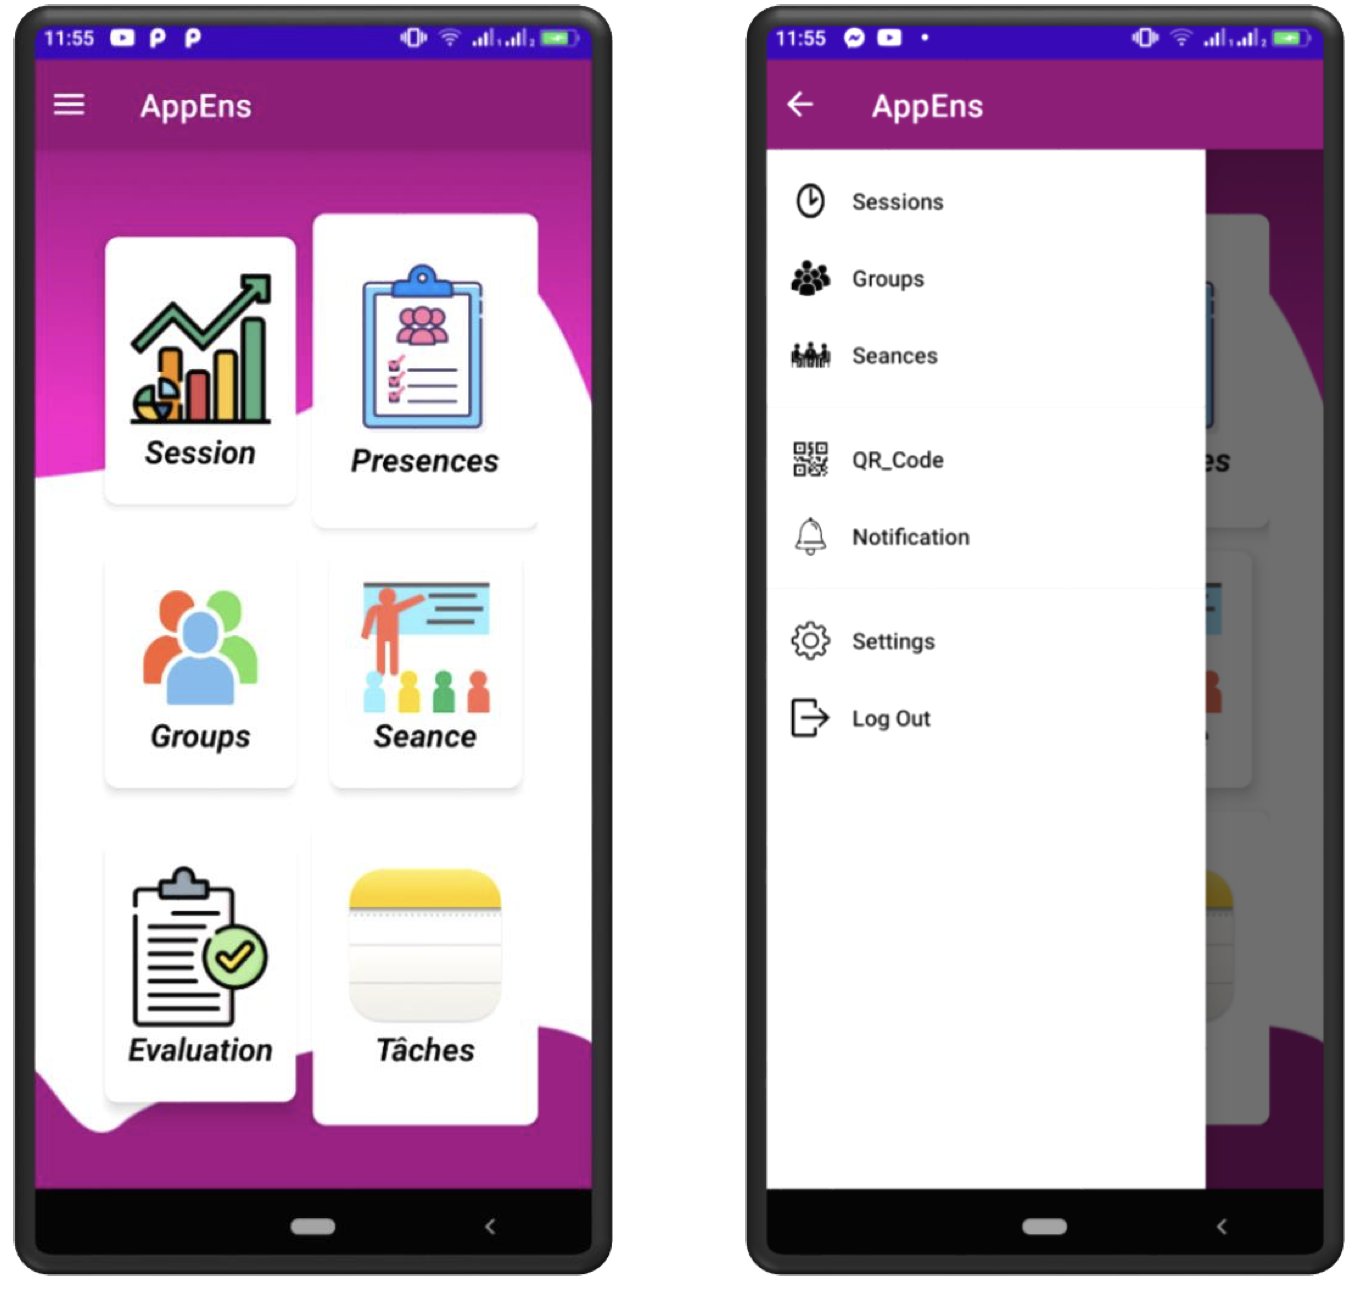
\includegraphics[width=0.8\textwidth]{images/morsli/rayane_jijel.png}
    \caption{Main Dashboard}
    \label{fig:attendance-system}
\end{figure}



\vspace{5cm}
\subsection{Example of a thesis from University of Ibn Khaldoun – Tiaret – Bachelor's Degree – 2013/2014
(realization of a software for managing student absences)}

This example represents a software for managing absences in the Department of Preparatory Studies at the School of Sciences and Technologies in Tlemcen (E.P.S.T.T).
This application offers several advantages, including faster search for information related to student absences, archiving data efficiently, and facilitating the retrieval of academic council decisions related to students.
Additionally, the program enhances data security, speeds up the execution of procedures, and contributes to more efficient management of absences and simplification of the related administrative operations ~\cite{mekki2014}.
Some of the interfaces are presented below.
\begin{figure}[htbp]
    \centering
    \begin{subfigure}[b]{0.45\textwidth}
        \centering
        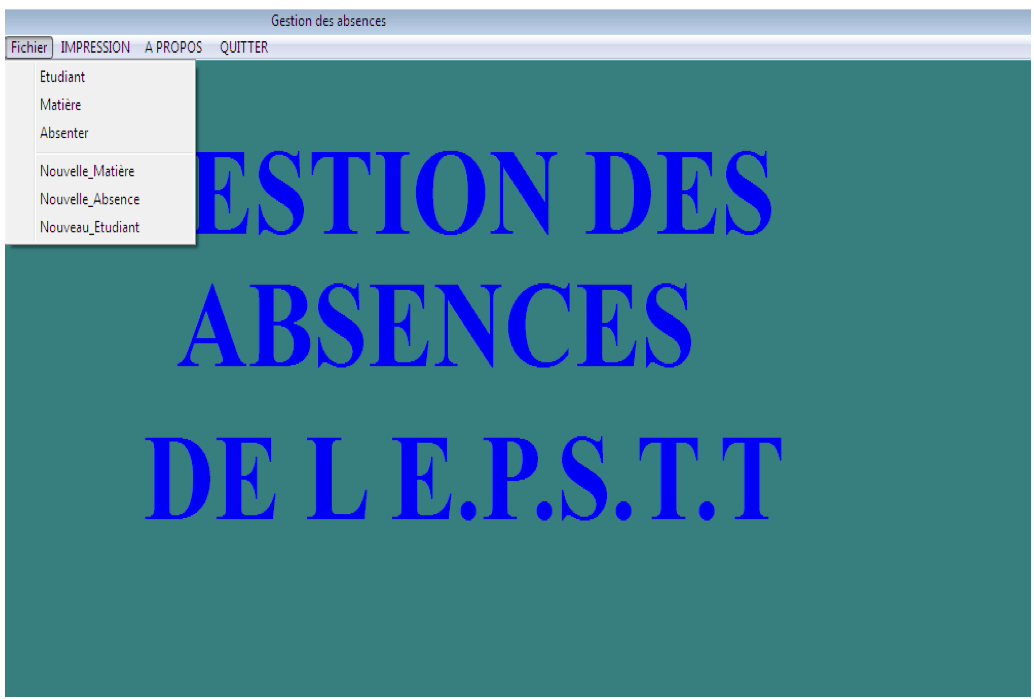
\includegraphics[width=\textwidth]{images/morsli/mekki1.png}
        \caption{Main Dashboard}
        \label{fig:dashboard}
    \end{subfigure}
    \hfill
    \begin{subfigure}[b]{0.45\textwidth}
        \centering
        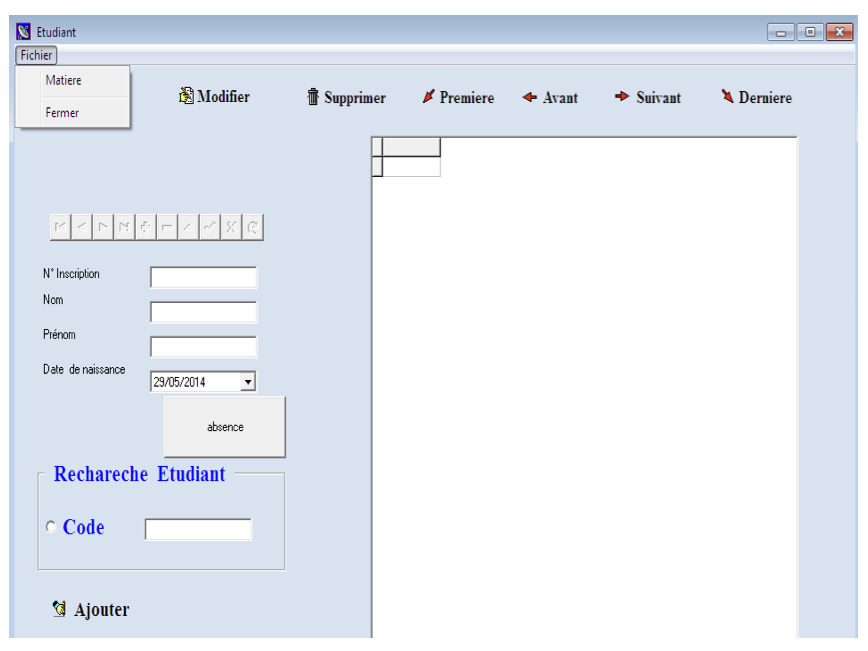
\includegraphics[width=\textwidth]{images/morsli/mekki2.png}
        \caption{Student}
        \label{fig:student}
    \end{subfigure}
    \caption{Dashboard and Student views}
    \label{fig:attendance-system}
\end{figure}

%\vspace{7cm}




\section{Proposed Solution}
To address the identified problem, this project proposes designing and developing a mobile application that allows students to register their attendance by scanning a unique QR Code assigned to each class using their smartphones. The QR code is pre-generated. Upon entering the classroom, the student scans the code from the teacher device, and their attendance is automatically recorded in a central database.

The system ensures the accuracy of entered data and prevents any attempts at manipulation by automatically recording the time and date of attendance. Students can only register their attendance when physically present in the designated location. Moreover, the system allows teachers to access real-time attendance data. The system's user interface is designed to be simple and intuitive, making it easy for all users to interact with it without requiring advanced technical skills.

This solution streamlines attendance tracking by reducing time and effort, improving accuracy, and enabling quick access to student data, ultimately enhancing educational management.

\section{Objectives}
This project aims to achieve a set of key objectives that contribute to improving the student attendance process and enhancing the performance of educational processes. These objectives include:

\begin{itemize}
    \item \textbf{Facilitating the attendance recording process:} By automating the attendance process using QR Code technology, teachers can efficiently record student presence without manual effort, reducing administrative workload and freeing up more time for teaching.
    \item \textbf{Ensuring the accuracy of attendance data:} Through the digital system, the likelihood of human errors or data manipulation is minimized, as the time and date of attendance are recorded automatically and accurately.
    \item \textbf{Enhancing the efficiency of educational processes:} By providing a centralized database that allows teachers to access and analyze attendance data at any time, facilitating the preparation of reports and supporting quick and informed decision-making.
    \item \textbf{Ensuring security and privacy:} The system is designed to maintain the confidentiality of student data and prevent unauthorized access, enhancing user trust and ensuring compliance with security standards.
\end{itemize}
\section{Conclusion}
In summary, the proposed mobile attendance tracking system based on QR Code technology presents a modern and effective solution to the limitations of traditional attendance methods. By automating the attendance process and centralizing data management, the system ensures greater accuracy, saves time, and enhances administrative efficiency within educational institutions. 

Through a detailed analysis of existing systems and the identification of key challenges, this project outlines a practical and scalable approach that meets the needs of both students and academic staff. The integration of user-friendly interfaces and secure data handling mechanisms further contributes to the system's reliability and ease of adoption.

This work not only supports the ongoing digital transformation in the education sector but also lays the groundwork for future enhancements, such as integration with learning management systems (LMS), advanced analytics, and geolocation-based verification. Ultimately, the implementation of this system has the potential to significantly improve the quality of educational services and foster a more efficient, transparent, and tech-savvy academic environment.



\newpage
\thispagestyle{empty}

\setcounter{chapter}{1} % Set to 1 so refstepcounter will increment to 2
\refstepcounter{chapter}

\phantomsection
\addcontentsline{toc}{chapter}{\protect\numberline{\thechapter}Theoretical Part}

\vspace*{\fill}
\begin{center}
    {\color{mintgreen} \rule{\textwidth}{2pt} }\\[0.5cm]
    {\Huge \textbf{Theoretical Part}}\\[0.5cm]
    {\color{mintgreen} \rule{0.8\textwidth}{1.5pt} }
\end{center}
\vspace*{\fill}

\begin{center}
    {\color{mintgreen} \rule{0.8\textwidth}{1.5pt} }\\[0.3cm]
    {\color{mintgreen} \rule{\textwidth}{2pt} }
\end{center}




\newpage
\vspace{0.3cm}
\refstepcounter{section}

\begin{tcolorbox}[
    colback=mintgreen!20, 
    colframe=mintgreen!80!black, 
    width=\textwidth, 
    boxrule=1pt, 
    arc=5pt, 
    auto outer arc,
    left=10pt,
    right=10pt,
    top=6pt,
    bottom=6pt
]
    \centering
    \Large \textbf{Section 1 : General Concepts} % ← manual label
\end{tcolorbox}

\phantomsection
\addcontentsline{toc}{section}{\protect\numberline{\thesection}General Concepts}

\subsection{Introduction}
In today's rapidly evolving digital landscape, the development of software systems has become a cornerstone of innovation across virtually every sector. From healthcare and education to logistics and finance, robust and scalable software solutions are essential for addressing complex problems and enhancing operational efficiency. In this context, designing and implementing an effective software system requires a structured and well-informed approach that bridges user needs with technical execution.

This section focuses on the foundational aspects of software conception as applied to the development of a QR Code-based attendance tracking system. The primary goal of this system is to streamline and secure the process of recording student attendance through the integration of mobile technologies and real-time data processing. To achieve this, a strong emphasis is placed on applying proven software engineering principles and modeling practices.

The following sections explore the general concepts underlying software design, with particular attention to object-oriented methodologies and the Unified Modeling Language (UML)~\cite{omg2017}. These approaches provide a systematic framework for translating functional requirements into a coherent software architecture that supports maintainability, scalability, and ease of use.


\subsection{Introduction to Software Conception}
Software conception is an essential step in the software development lifecycle. It occurs between requirements analysis and the coding phase, and constitutes a fundamental transition between what the software should do and how it will do it. This step allows for defining the global architecture of the system, its components, the interfaces between them, and the technological choices to adopt. The main objective is to design a software solution that is robust, efficient, scalable, and easy to maintain.

According to Ian Sommerville in \textit{Software Engineering} (10\textsuperscript{th} edition), good design should respect principles such as modularity, separation of concerns, low coupling between modules, and high internal cohesion~\cite{sommerville2015}. These principles facilitate code reuse, testing, maintenance, and reduce the risk of errors during development.

Pressman and Maxim, in their reference work \textit{Software Engineering: A Practitioner's Approach}, emphasize the importance of object-oriented design, which models the system as a collection of objects interacting via messages, more accurately representing the reality of the application world~\cite{pressman2014}.

\subsection{Software Conception Models}
Before detailing the UML language, it is important to note that there are several approaches and software design models that allow representing the functioning of a system. Among the most well-known, we can cite:

\begin{itemize}
  \item \textbf{The Waterfall model}: a sequential approach where each phase of development must be completed before moving on to the next ~\cite{royce1970}.
  \item \textbf{The Spiral model}: based on an iterative and incremental approach integrating risk analysis ~\cite{boehm1988}.
  \item \textbf{The Agile model}: an iterative and evolutionary method centered on collaboration, frequent deliverables, and continuous adaptation to needs ~\cite{beck2001, cockburn2002}.
  \item \textbf{Object-oriented design}: it consists of modeling a system in terms of objects, classes, and interactions, approaching the way we perceive the real world ~\cite{booch1994, gamma1995}.
\end{itemize}

These models influence the choice of modeling tools. For this project, we opted for object-oriented design and the use of UML language due to its expressive richness, international standardization \cite{omg2017}, and widespread adoption in industrial and academic projects \cite{rumbaugh2004, fowler2004}.


\subsection{Definition of UML (Unified Modeling Language)}
The Unified Modeling Language (UML) is a standardized graphical language used for modeling software systems. It offers a set of standardized notations allowing visual representation of different views of a system: static structure, dynamic behavior, interactions, use cases, etc.
Initially designed by Grady Booch, James Rumbaugh, and Ivar Jacobson (often referred to as "the Three Amigos") at Rational Software in the mid-1990s, UML was standardized by the OMG (Object Management Group) in 1997~\cite{omg2017}. UML emerged as a unification of several object-oriented modeling approaches that were prevalent during that period, creating a common visual language for software developers worldwide~\cite{pressman2014}.
UML version 2.5.1, released in 2017, includes 14 types of diagrams divided into three major categories:
\begin{itemize}
\item Structural diagrams (e.g., class diagram, component diagram, object diagram, package diagram, deployment diagram, composite structure diagram, profile diagram),
\item Behavioral diagrams (e.g., activity diagram, state diagram, use case diagram),
\item Interaction diagrams (e.g., sequence diagram, communication diagram, timing diagram, interaction overview diagram).
\end{itemize}
Each diagram type serves a specific purpose in the software development lifecycle. For instance, class diagrams represent the static structure of a system by showing classes, their attributes, methods, and relationships, while sequence diagrams illustrate the dynamic interactions between objects over time~\cite{sommerville2015}. This multi-perspective approach enables comprehensive modeling of complex software systems from different viewpoints.
UML promotes shared understanding among stakeholders (developers, analysts, clients, etc.) and improves system documentation~\cite{omg2017}. As noted by Sommerville, "UML has become the standard language for describing and documenting object-oriented systems"~\cite{sommerville2015}. Its widespread adoption across the software industry has established it as a lingua franca for software architects and developers.
The flexibility of UML allows it to be used in various software development methodologies, from traditional plan-driven approaches to agile methods. In agile contexts, lightweight UML modeling often focuses on select diagram types to communicate essential system aspects without excessive documentation overhead~\cite{pressman2014}. Conversely, in more formal development environments, UML can be applied rigorously to produce detailed system specifications.
Beyond its core diagramming capabilities, UML also supports model-driven development through the Object Constraint Language (OCL) and various profile extensions that adapt UML to specific domains or platforms. These extensions enhance UML's utility across diverse application domains, including real-time systems, web applications, and enterprise software~\cite{omg2017}.
Despite criticisms regarding its complexity and learning curve, UML remains a cornerstone of software engineering education and practice, providing a standardized visual vocabulary that transcends programming languages and implementation technologies~\cite{sommerville2015}.

\vspace{3cm}


\newpage
\vspace{0.3cm}
\refstepcounter{section}

\begin{tcolorbox}[
    colback=mintgreen!20, 
    colframe=mintgreen!80!black, 
    width=\textwidth, 
    boxrule=1pt, 
    arc=5pt, 
    auto outer arc,
    left=10pt,
    right=10pt,
    top=6pt,
    bottom=6pt
]
    \centering
    \Large \textbf{Section 2 : System Modeling} % ← manual label
\end{tcolorbox}

\phantomsection
\addcontentsline{toc}{section}{\protect\numberline{\thesection}System Modeling}

\subsection{Introduction}
To better understand, design, and communicate the structure and behavior of the attendance tracking system, we employ Unified Modeling Language (UML) diagrams. UML provides a standardized visual notation that aids both technical and non-technical stakeholders in grasping system components and interactions. The following subsections present three essential UML diagrams : use case diagram, class diagram, activity diagram and sequence diagram ,each focusing on a different aspect of the system's design.

\subsection{Use Case Diagram}
The use case diagram illustrates the core functionalities of the student attendance system from the perspective of its primary users. It highlights the external \textit{actors} and \textit{use cases}, offering a clear view of how users interact with the system and what operations they can perform ~\cite{fowler2004}.

\textbf{Main Actors :}
\begin{itemize}
\item The \textbf{teacher}, who is responsible for generating QR codes for each session, monitoring student attendance, and viewing class details.
\item The \textbf{student}, who scans the QR code to mark their presence, views their attendance history, and can submit an excuse in case of absence.
\end{itemize}

\textbf{ Some use Cases :}
\begin{itemize}
\item Authentication (Teacher , Student),
\item QR code generation and scanning (Teacher),
\item Attendance monitoring and viewing (Teacher),
\item Absence justification submission (Student).
\end{itemize}

The use case diagram illustrating these interactions is shown right below.
\begin{figure}[htbp]
    \centering
    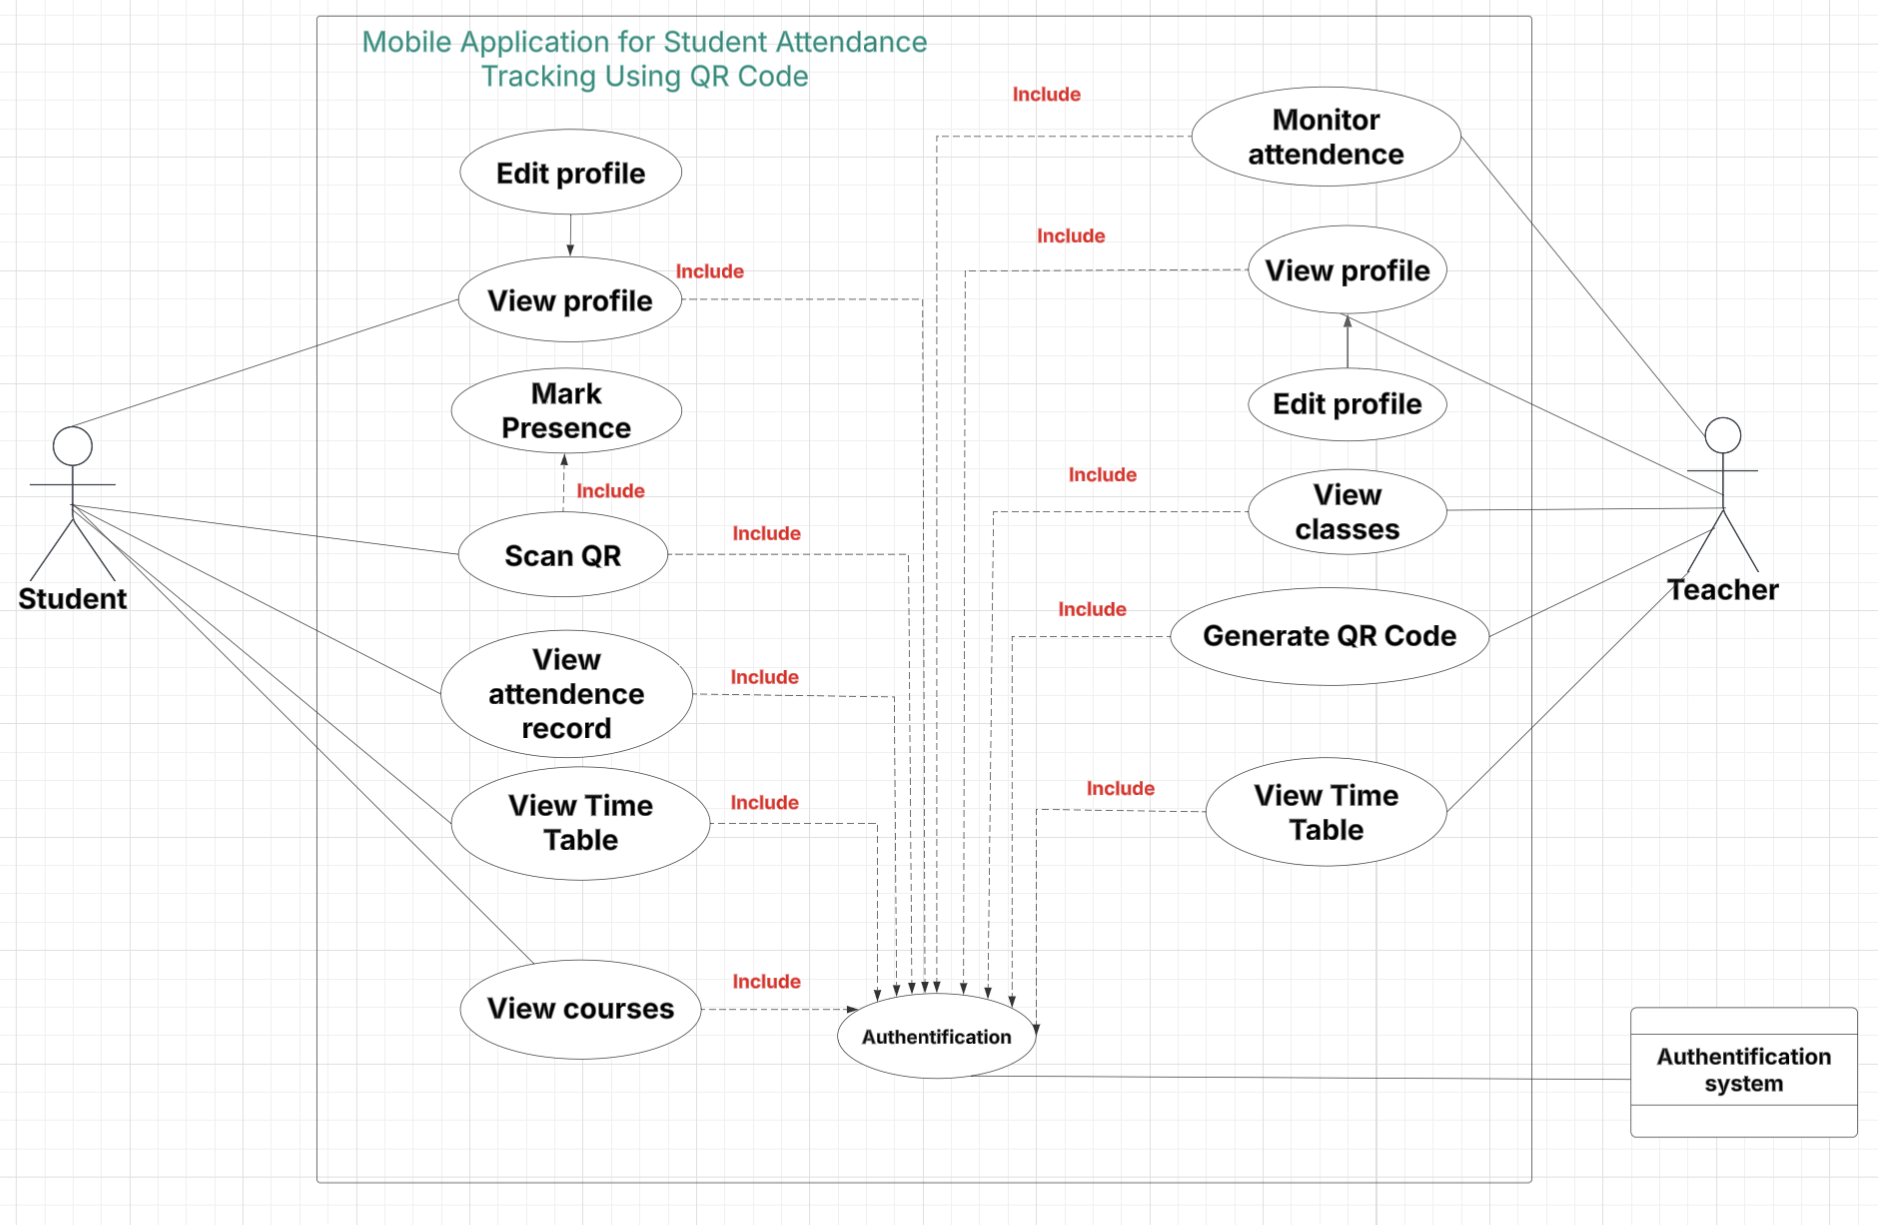
\includegraphics[width=0.8\textwidth]{images/morsli/use_case2.png}
    \caption{Use Case Diagram}
    \label{fig:attendance-system}
\end{figure}

\vspace{9,5cm}
\newline
This diagram offers an overview of system functionalities, understandable even by non-technical users~\cite{fowler2004}.

\subsection{Class Diagram}
The class diagram is a structural diagram that describes the system's object classes, their attributes, operations, and the relationships (associations, inheritances, dependencies) between them ~\cite{fowler2004}.

\textbf{Examples of Classes:}
\begin{itemize}
  \item \texttt{Profile}: id, first\_name, last\_name, role, phone,
  \item \texttt{Student\_Profile}: id, profile\_id, student\_group\_id, student\_id,
  \item \texttt{Teacher\_Profile}: id, profile\_id, department\_id, employee\_id,
  \item \texttt{Session}: id, schedule\_id, start\_time, end\_time, status,
  \item \texttt{Attendance}: id, session\_id, student\_id, timestamp, status.
\end{itemize}


\begin{table}[H]
\centering
\small % Smaller text size for better fit
\caption{Explanation of Classes in the Class Diagram}
\renewcommand{\arraystretch}{1.3}
\begin{tabular}{|p{3cm}|p{4cm}|p{7.5cm}|}
\hline
\textbf{Class Name} & \textbf{Key Attributes} & \textbf{Description} \\
\hline
\texttt{profiles} & \texttt{id}, \texttt{first\_name}, \texttt{last\_name}, \texttt{role}, \texttt{phone} & Base profile information for all users (admin, student, teacher). \\
\hline
\texttt{departments} & \texttt{id}, \texttt{name}, \texttt{code} & Represents academic departments to which users and courses belong. \\
\hline
\texttt{admin\_profiles} & \texttt{id}, \texttt{profile\_id}, \texttt{department\_id} & Links an admin profile to the general profile and their department. \\
\hline
\texttt{teacher\_profiles} & \texttt{id}, \texttt{profile\_id}, \texttt{department\_id}, \texttt{employee\_id} & Defines a teacher, extending \texttt{profiles} with department and employee data. \\
\hline
\texttt{student\_groups} & \texttt{id}, \texttt{department\_id}, \texttt{academic\_year}, \texttt{section}, \texttt{name} & Groups students by year, section, and department. \\
\hline
\texttt{student\_profiles} & \texttt{id}, \texttt{profile\_id}, \texttt{student\_group\_id}, \texttt{student\_id} & Represents individual student profiles linked to their group and main profile. \\
\hline
\texttt{courses} & \texttt{id}, \texttt{title}, \texttt{description}, \texttt{credit\_hours}, \texttt{semester} & Academic courses with details such as credits and semester. \\
\hline
\texttt{group\_courses} & \texttt{id}, \texttt{course\_id}, \texttt{student\_group\_id}, \texttt{academic\_year} & Assigns courses to student groups. \\
\hline
\texttt{teacher\_course\_groups} & \texttt{id}, \texttt{teacher\_id}, \texttt{course\_id}, \texttt{student\_group\_id}, \texttt{academic\_year} & Links teachers to the student groups and courses they teach. \\
\hline
\texttt{time\_slots} & \texttt{id}, \texttt{start\_time}, \texttt{end\_time}, \texttt{day\_of\_week} & Defines recurring schedule slots by day and time. \\
\hline
\texttt{weekly\_schedule} & \texttt{id}, \texttt{time\_slot\_id}, \texttt{teacher\_id}, \texttt{course\_id}, \texttt{student\_group\_id}, \texttt{room\_number} & Weekly teaching schedule linking time slots to teachers and groups. \\
\hline
\texttt{sessions} & \texttt{id}, \texttt{schedule\_id}, \texttt{start\_time}, \texttt{end\_time}, \texttt{status} & Instances of scheduled sessions (lessons) to track attendance. \\
\hline
\texttt{attendance} & \texttt{id}, \texttt{session\_id}, \texttt{student\_id}, \texttt{timestamp}, \texttt{status} & Records whether a student was present, absent, or justified for a session. \\
\hline
\end{tabular}
\end{table}



\begin{figure}[htbp]
    \centering
    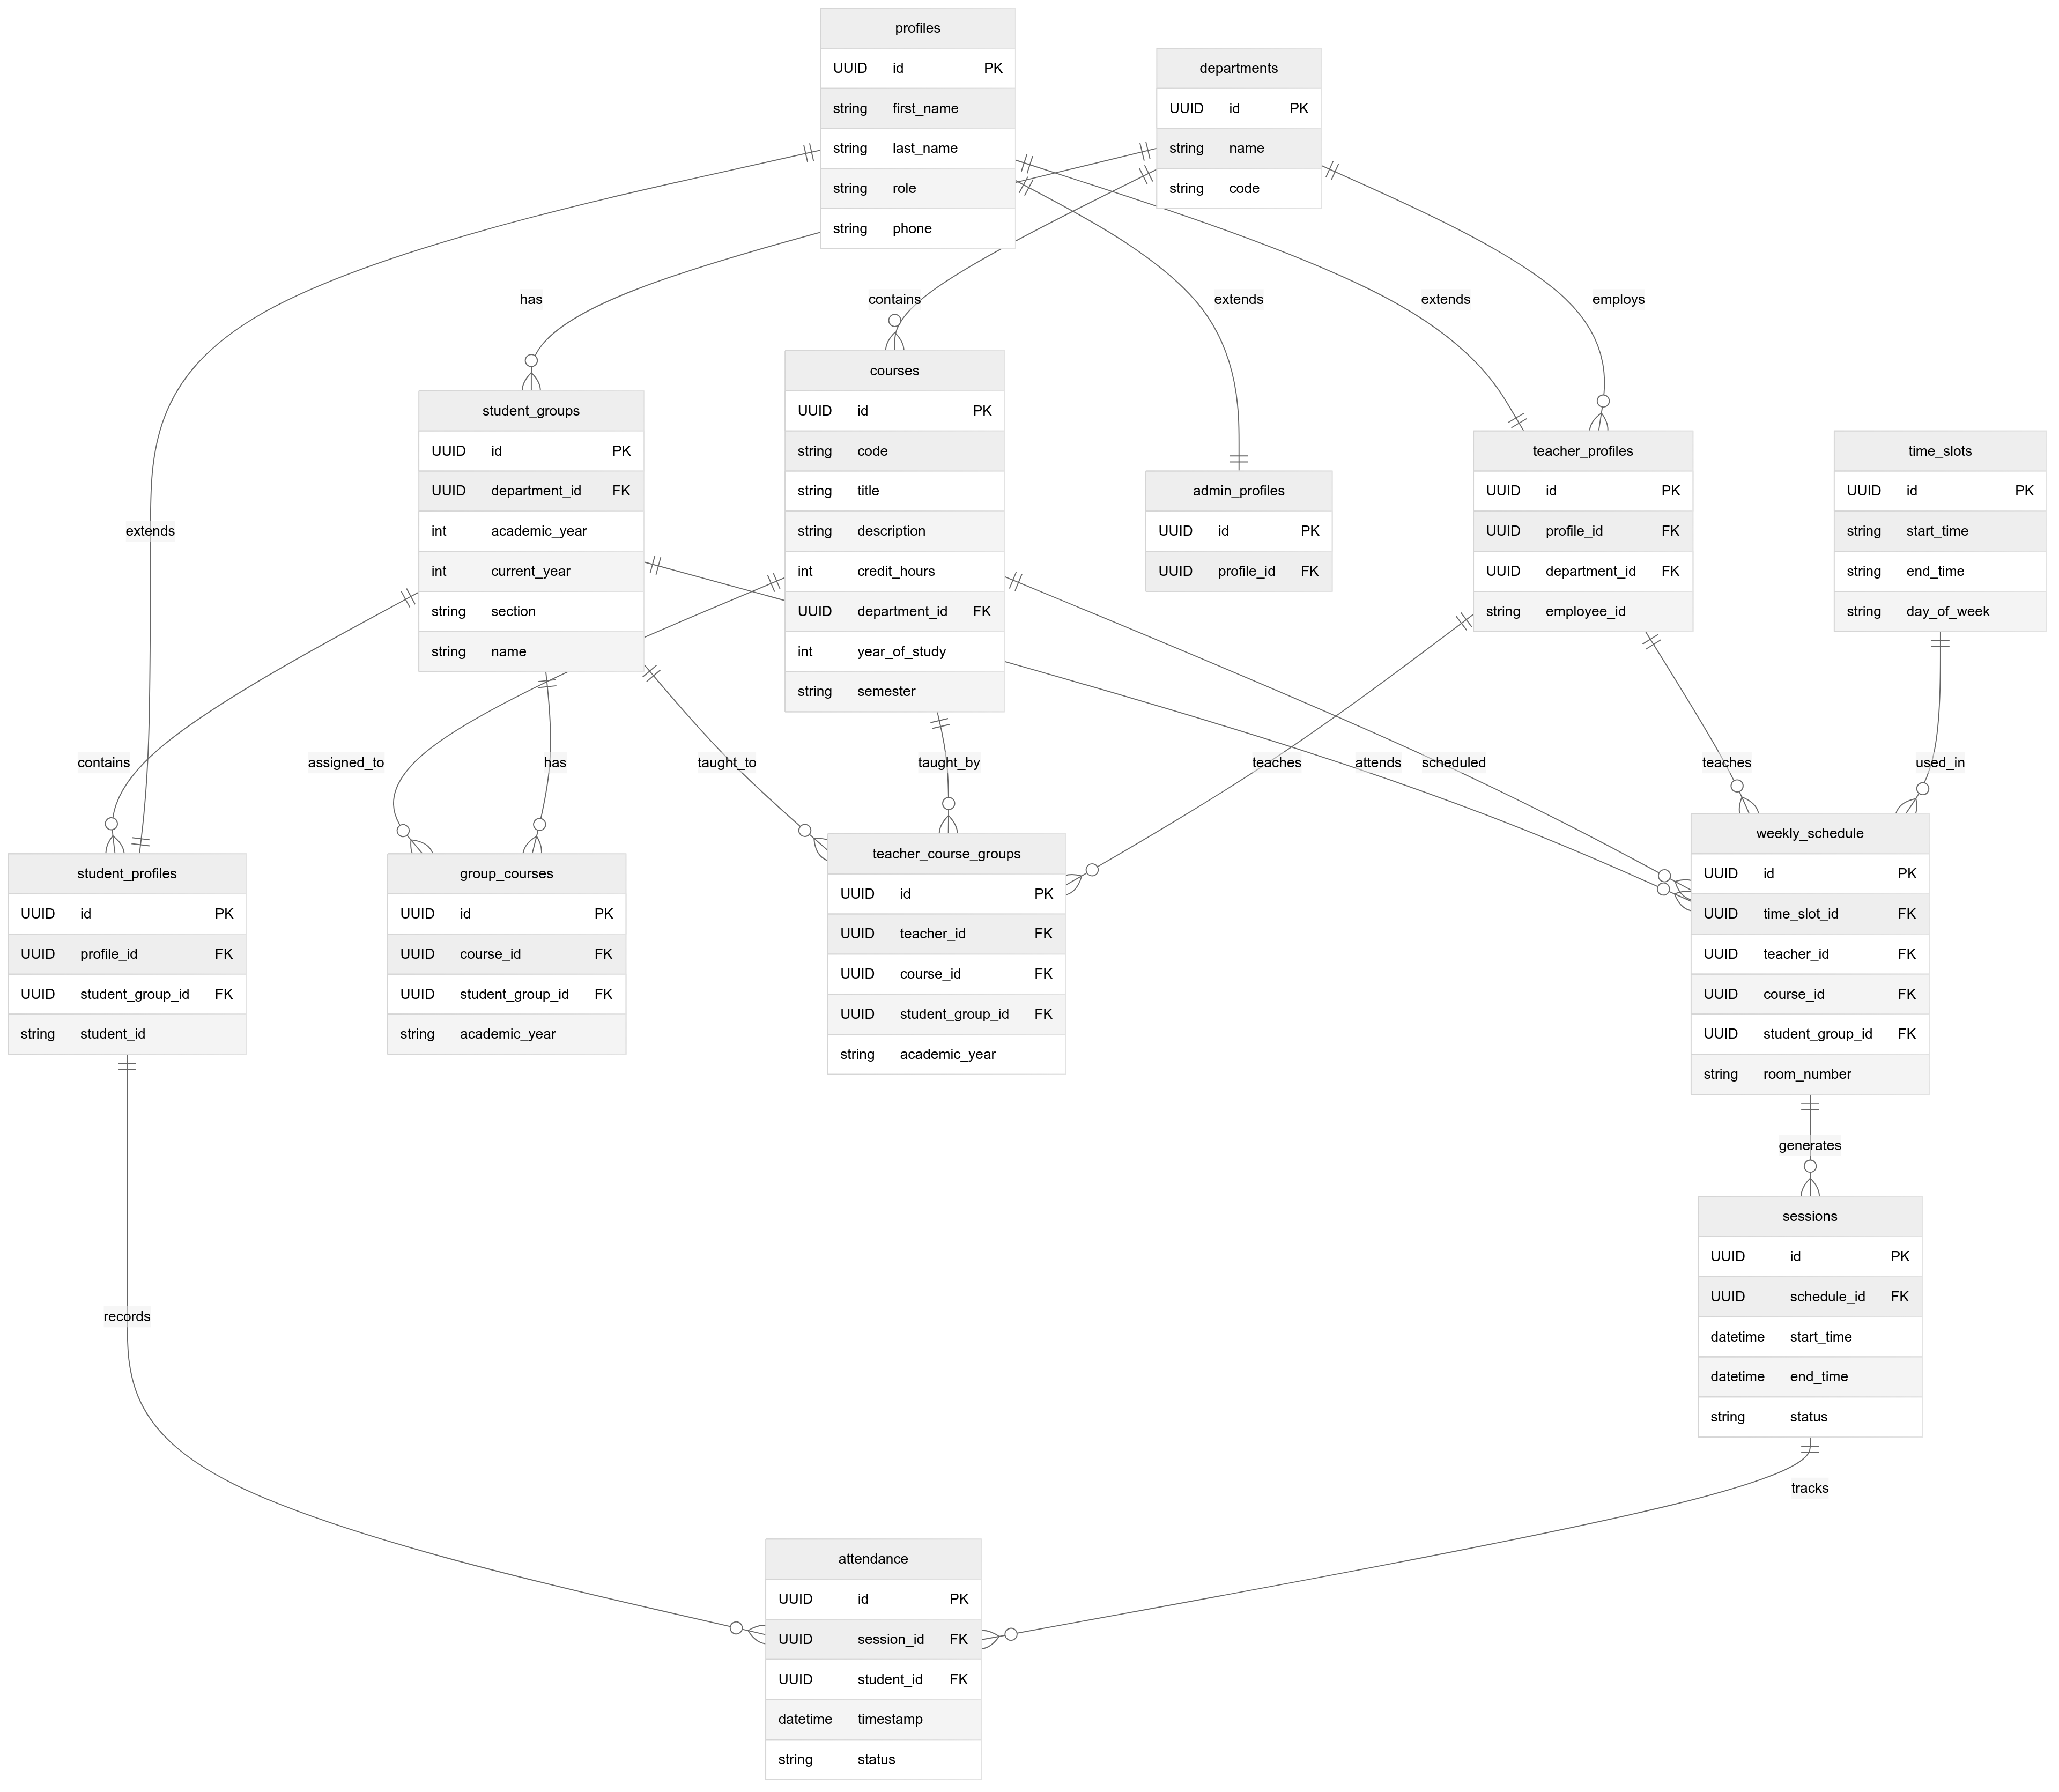
\includegraphics[width=0.8\textwidth]{images/morsli/class_diagram.png}
    \caption{Class Diagram}
    \label{fig:attendance-system}
\end{figure}

This diagram facilitates database structuring and guides object-oriented implementation~\cite{bruegge2010}.


\newpage
\subsection{Activity Diagram}
The activity diagram models the workflow of a business process. It allows representing the different steps, decisions, parallelisms, and conditions of a business or software process~\cite{fowler2004}.

\textbf{Example of Role-Based Access Scenario:}
\begin{enumerate}
\item The user opens the application,
\item They enter their credentials,
\item The system authenticates the user,
\item The system checks the user’s role (e.g., Teacher, Student, or No Role),
\item If no role is found, the user is redirected to the login screen,
\item If the user is a Teacher:
\begin{itemize}
\item The Teacher Role Guard verifies their access,
\item If authorized, they access the Teacher Features,
\item If unauthorized, they are redirected to the login screen,
\end{itemize}
\item If the user is a Student:
\begin{itemize}
\item The Student Role Guard verifies their access,
\item If authorized, they access the Student Features,
\item If unauthorized, they are redirected to the login screen.
\end{itemize}
\end{enumerate}
This diagram allows optimizing interactions and identifying bottlenecks~\cite{arlow2005}.

The activity diagrams are shown right below.
\begin{figure}[htbp]
    \centering
    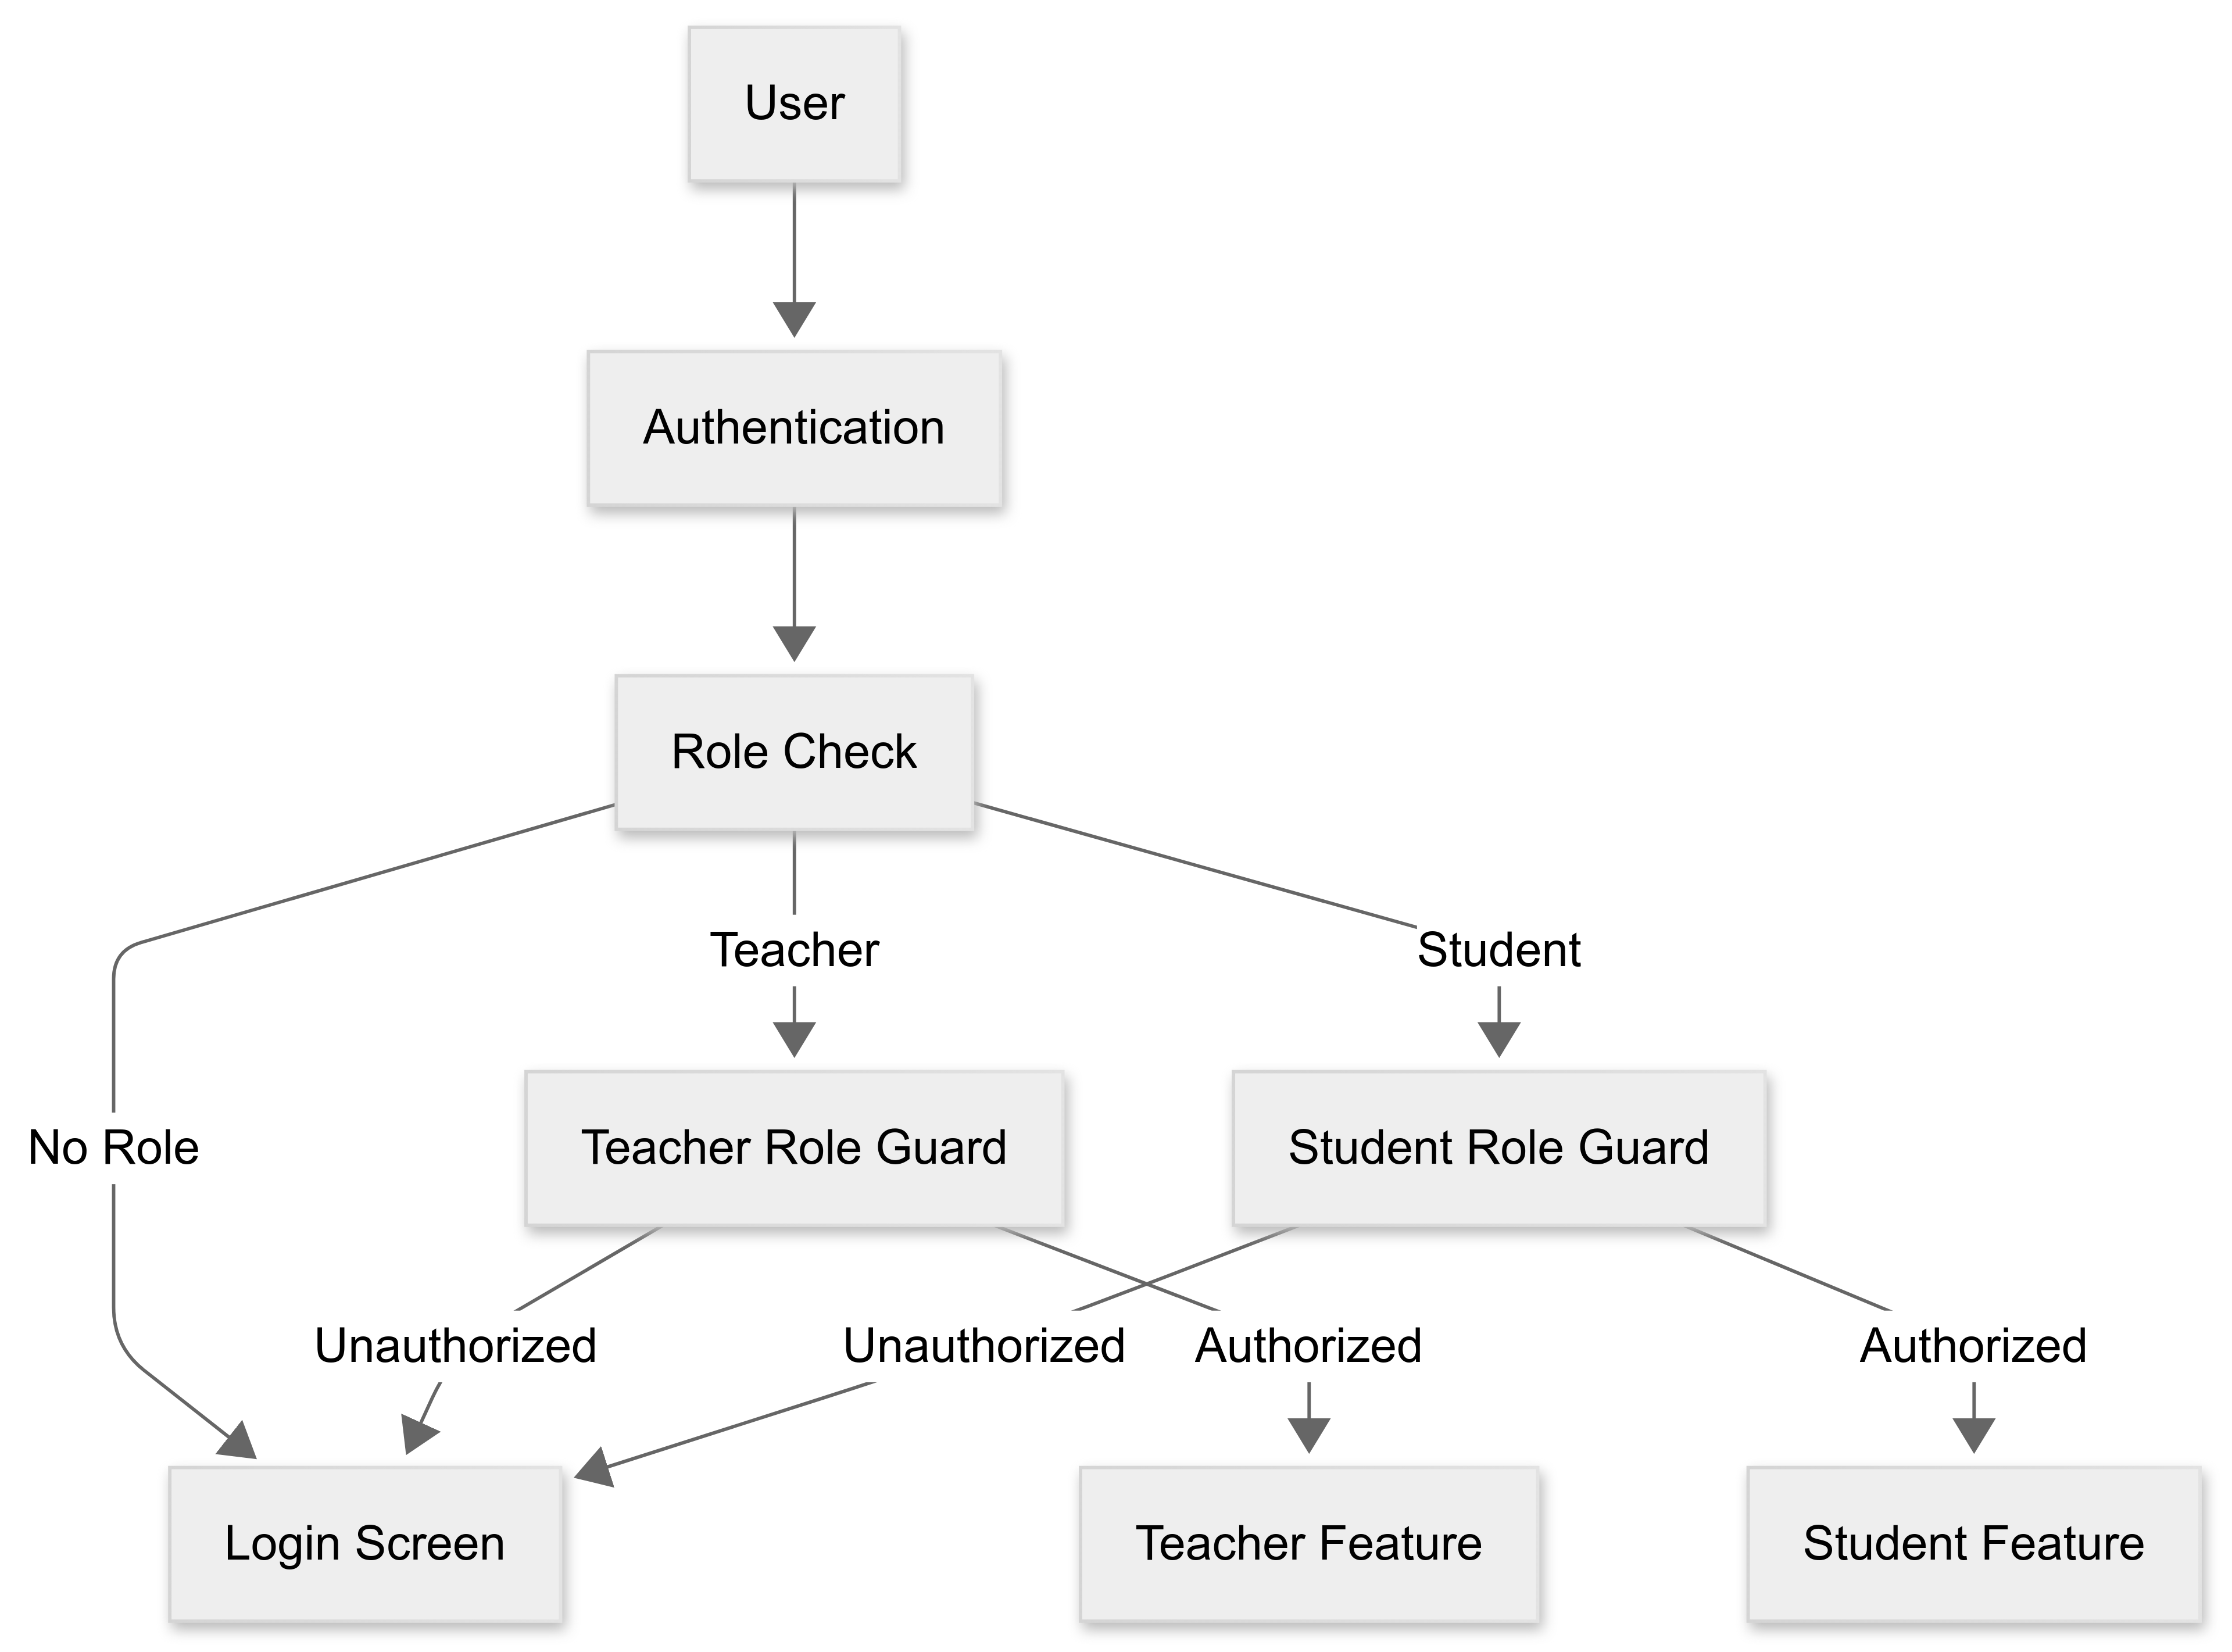
\includegraphics[width=0.8\textwidth]{images/morsli/Activity1.png}
    \caption{Authentification Activity Diagram}
    \label{fig:attendance-system}
\end{figure}

\vspace{20cm}

\begin{figure}[htbp]
    \centering
    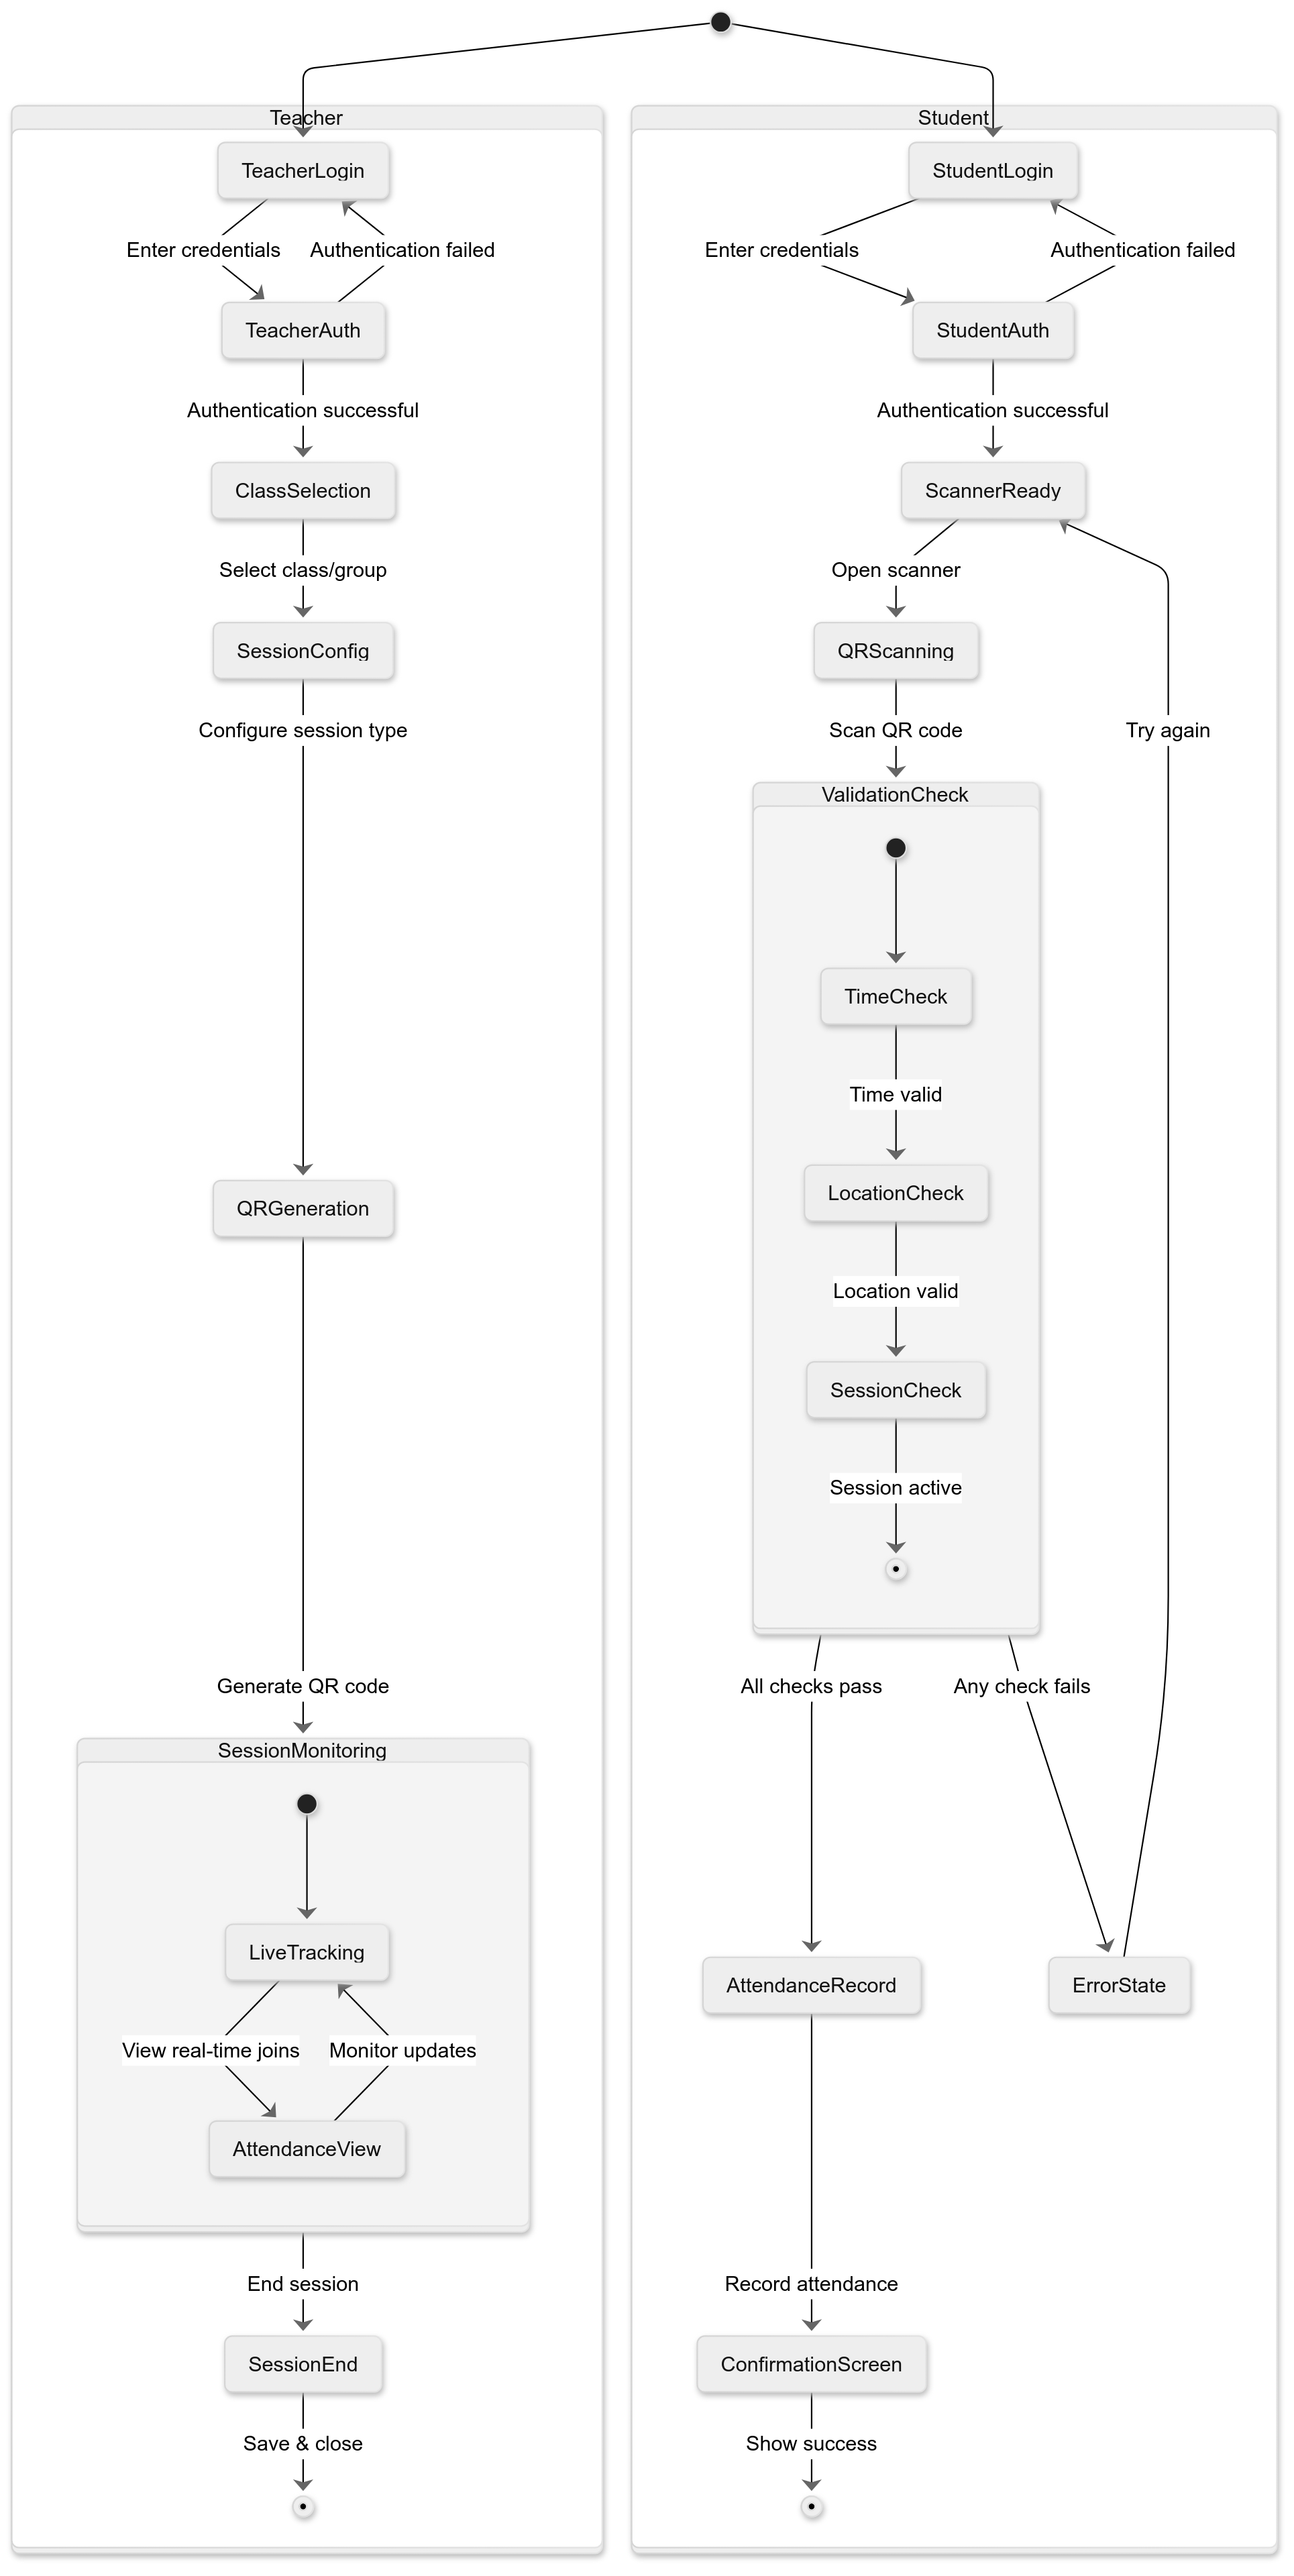
\includegraphics[width=0.8\textwidth]{images/morsli/Activity2.png}
    \caption{Teacher and Student Activity Diagram}
    \label{fig:attendance-system}
\end{figure}




\newpage
\subsection{Sequence Diagram}

A sequence diagram is a type of interaction diagram that shows how processes operate with one another and in what order. It visually represents the sequence of messages exchanged between different entities (objects or components) in a specific time sequence, focusing on the flow of logic within a system~\cite{booch2005uml}
.

\begin{figure}[htbp]
    \centering
    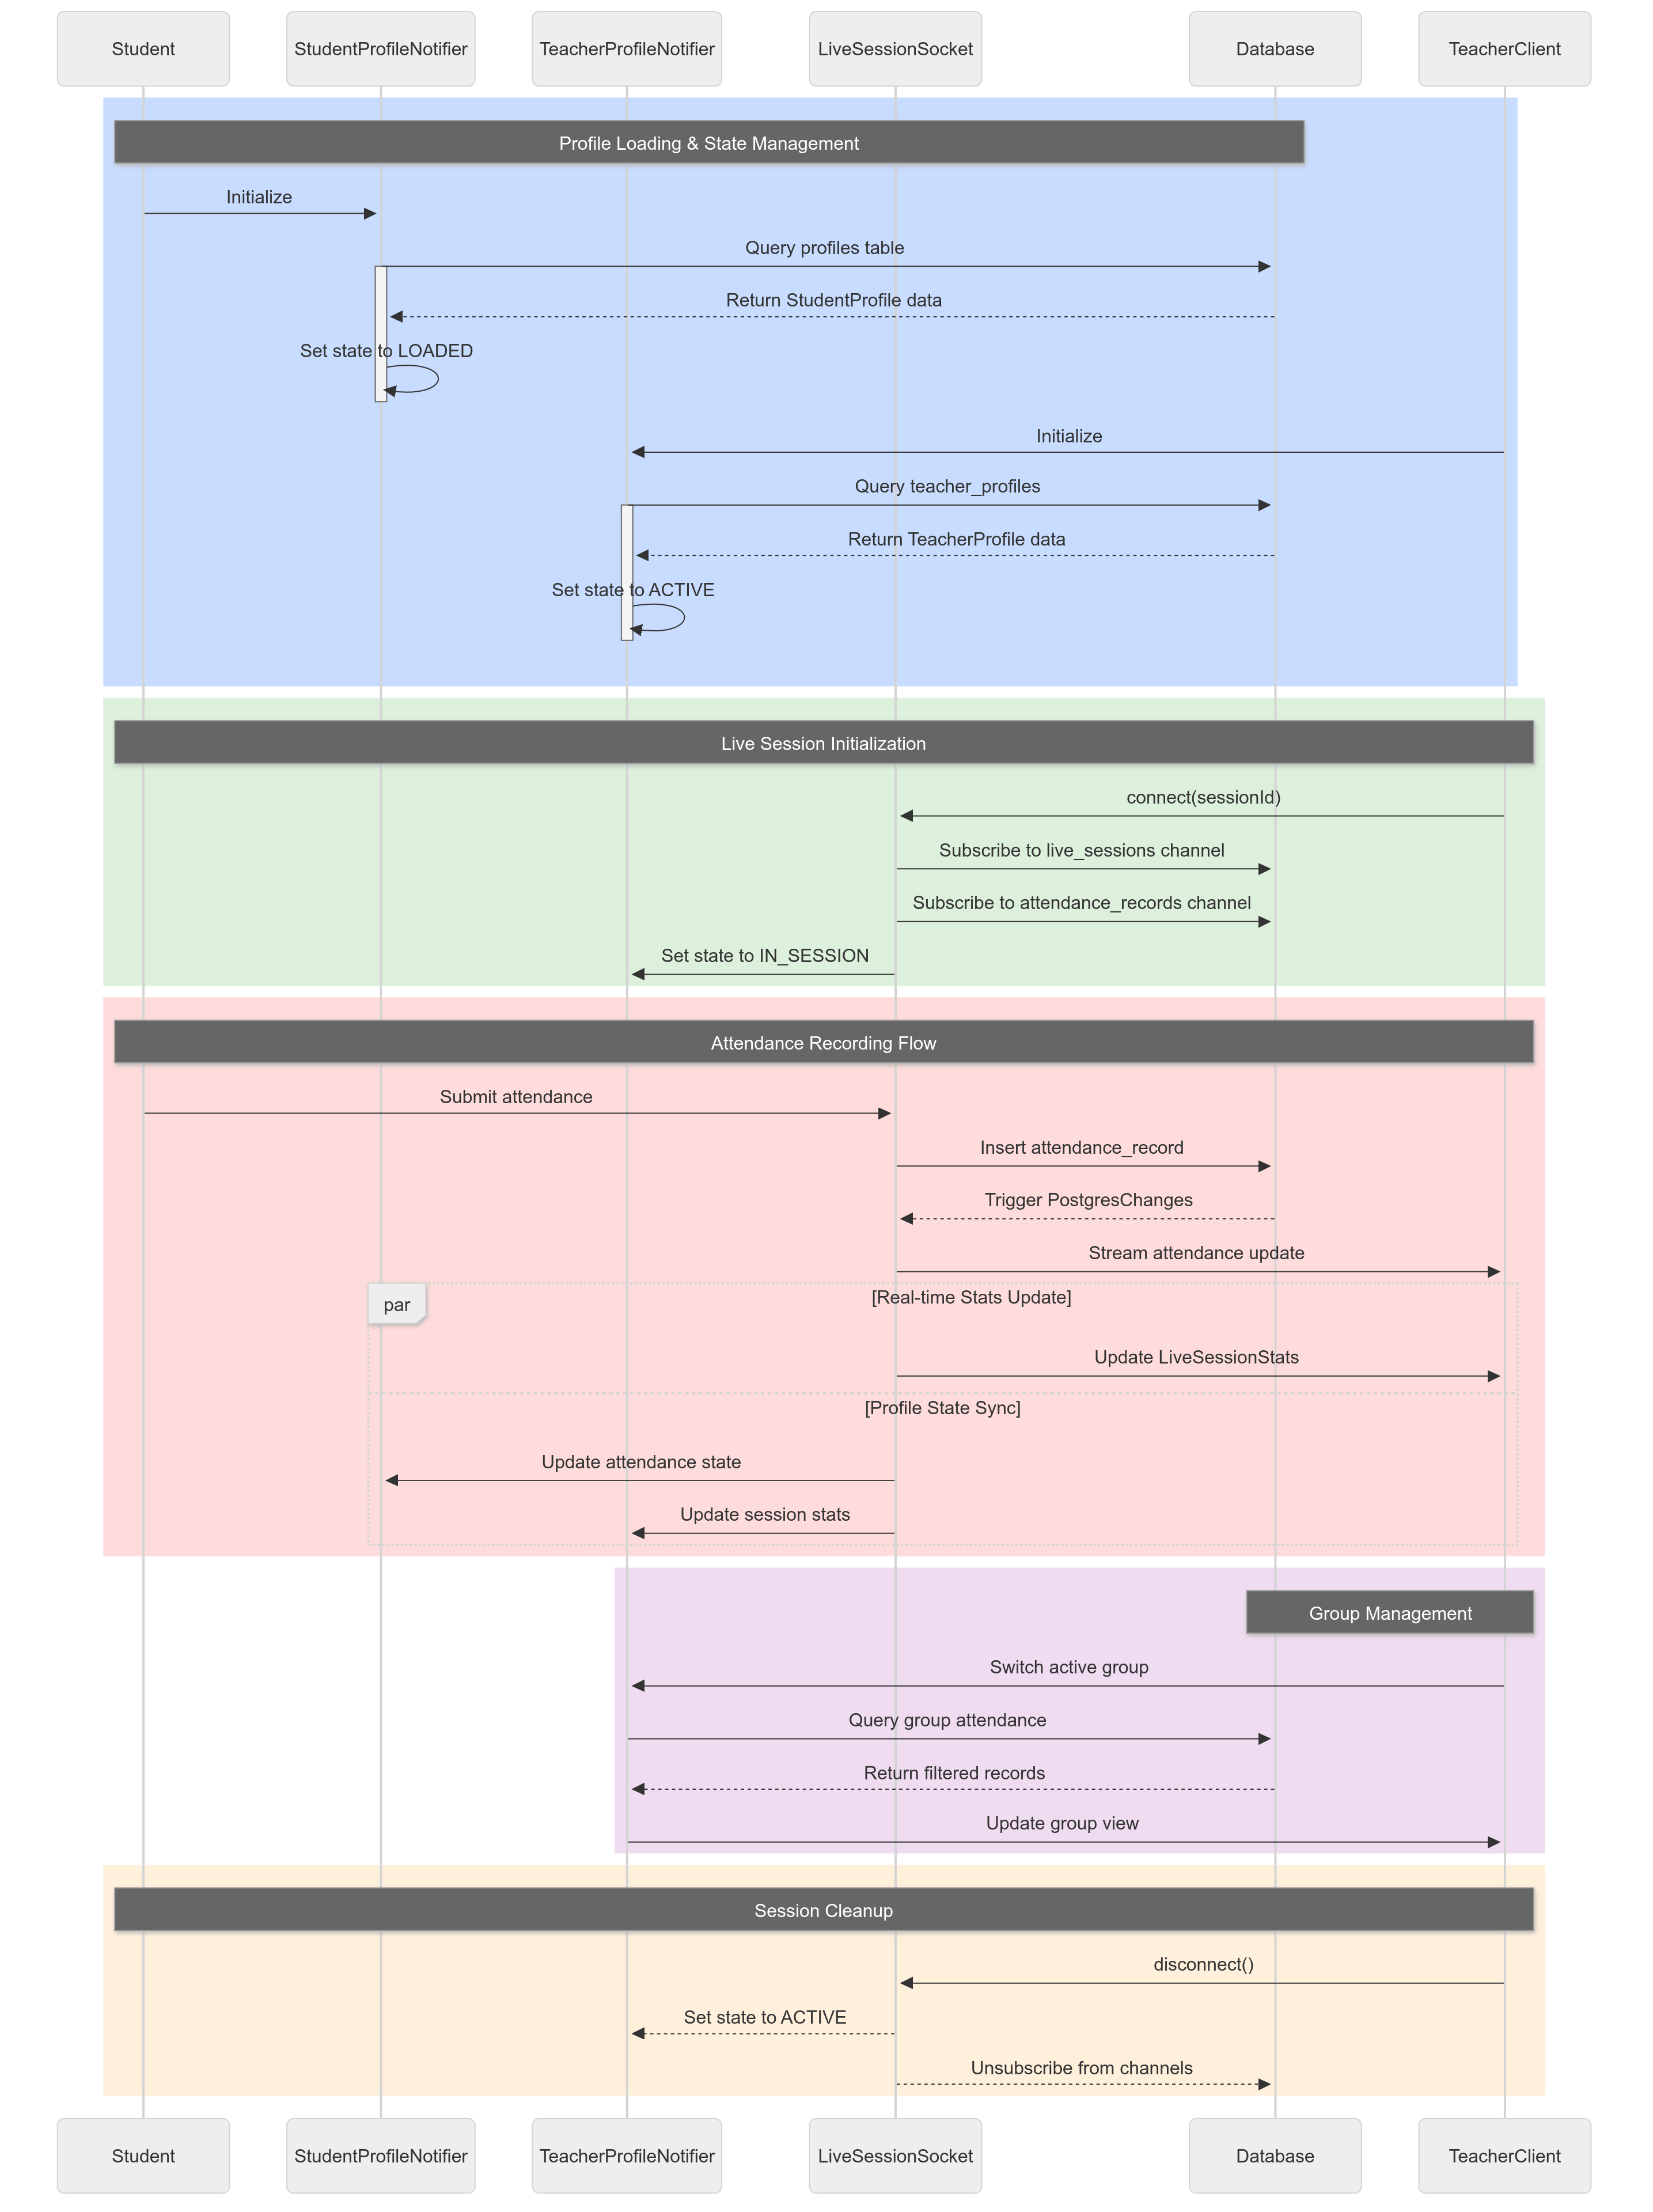
\includegraphics[width=0.8\textwidth]{images/morsli/sequence.png}
    \caption{Sequence Diagram}
    \label{fig:attendance-system}
\end{figure}

\textbf{Example of Attendance System Workflow:}

The sequence diagram illustrates the lifecycle of a live session in the attendance system. The key phases are:

\begin{enumerate}
    \item \textbf{Profile Loading \& State Management:}  
    The \textit{Student} and \textit{TeacherClient} initialize by querying the profile tables. Once the data is received, the respective notifiers update the state to \texttt{LOADED} or \texttt{ACTIVE}.
    
    \item \textbf{Live Session Initialization:}  
    The client connects using a session ID and subscribes to both the live sessions and attendance records channels through the \textit{LiveSessionSocket}. Upon success, the state changes to \texttt{IN\_SESSION}.
    
    \item \textbf{Attendance Recording Flow:}  
    The student submits attendance, which inserts a record into the database. A PostgreSQL trigger streams the update, and real-time session stats are updated in parallel, along with the profile's attendance state.
    
    \item \textbf{Group Management:}  
    The teacher can switch between groups, triggering a query for attendance data. Filtered results are returned and used to update the group view.
    
    \item \textbf{Session Cleanup:}  
    The client disconnects and unsubscribes from the channels. The session state is reset to \texttt{ACTIVE}.
\end{enumerate}


\section{Conclusion}

In conclusion, understanding software conception and its associated models is fundamental to developing reliable, maintainable, and scalable systems. The transition from abstract requirements to concrete implementation begins with a well-thought-out design phase, guided by principles such as modularity, cohesion, and low coupling. Among various modeling paradigms, object-oriented design stands out for its alignment with real-world abstractions and its ability to efficiently structure complex systems.

In this project, several UML diagrams were employed to design and visualize the QR Code-based attendance tracking system. The \textit{use case diagram} clarified the core functionalities from the users’ perspectives. The \textit{class diagram} outlined the system's structural components and their relationships. The \textit{sequence diagram} captured the dynamic interactions during a live attendance session, and the \textit{activity diagram} modeled the workflow for access control and session participation. Together, these diagrams offered a comprehensive understanding of both the static and dynamic aspects of the system.

The Unified Modeling Language (UML) thus played a central role in ensuring clarity, consistency, and effective communication throughout the development process. By leveraging these models, this project laid a solid foundation for the implementation of a robust and user-friendly attendance system based on QR code technology.


\newpage
\thispagestyle{empty}

\setcounter{chapter}{2} % Set to 1 so refstepcounter will increment to 2
\refstepcounter{chapter}

\phantomsection
\addcontentsline{toc}{chapter}{\protect\numberline{\thechapter}Practical Part}

\vspace*{\fill}
\begin{center}
    {\color{mintgreen} \rule{\textwidth}{2pt} }\\[0.5cm]
    {\Huge \textbf{Practical Part}}\\[0.5cm]
    {\color{mintgreen} \rule{0.8\textwidth}{1.5pt} }
\end{center}
\vspace*{\fill}

\begin{center}
    {\color{mintgreen} \rule{0.8\textwidth}{1.5pt} }\\[0.3cm]
    {\color{mintgreen} \rule{\textwidth}{2pt} }
\end{center}

\section{Technical Implementation}

\subsection{Technology Stack}
The project is built using a modern and robust technology stack that ensures scalability, real-time capabilities, and a smooth user experience:

\subsubsection{Flutter Framework}
Flutter serves as the primary framework for building the cross-platform application, offering several key advantages:
\begin{itemize}
    \item Cross-platform development capability for Android, iOS, and web platforms
    \item Rich set of customizable widgets for building responsive UIs
    \item Hot reload feature for rapid development
    \item High performance with native compilation
    \item Version: SDK $\geq$ 3.1.3
\end{itemize}

\subsubsection{Supabase Backend}
Supabase (version 2.6.3) is utilized as the backend solution, providing:
\begin{itemize}
    \item Real-time database capabilities
    \item Built-in authentication system
    \item Powerful PostgreSQL database
    \item Real-time subscriptions for live updates
    \item Secure API access
\end{itemize}

\subsubsection{Key Dependencies}
The application leverages several essential packages:
\begin{itemize}
    \item \texttt{flutter\_riverpod} (v2.4.9): State management solution
    \item \texttt{qr\_flutter} (v4.1.0): QR code generation
    \item \texttt{qr\_code\_scanner\_plus} (v2.0.10): QR code scanning
    \item \texttt{flutter\_speed\_dial} (v7.0.0): Advanced floating action button
    \item \texttt{fl\_chart} (v0.66.2): Data visualization
    \item \texttt{web\_socket\_channel} (v2.4.0): Real-time communication
\end{itemize}

\subsection{Hardware and Software Requirements}

\subsubsection{Hardware Requirements}
\begin{itemize}
    \item Smartphone or tablet with camera capability for QR scanning
    \item Minimum 2GB RAM recommended
    \item At least 100MB of storage space
    \item Internet connectivity (WiFi or mobile data)
\end{itemize}

\subsubsection{Software Requirements}
\begin{itemize}
    \item Android: Android 5.0 (API level 21) or higher
    \item iOS: iOS 11.0 or higher
    \item Web browsers: Latest versions of Chrome, Firefox, Safari, or Edge
    \item Internet connection for real-time features
\end{itemize}

\clearpage
\subsection{Implementation Details}

\subsubsection{System Architecture}
The application follows a clean architecture pattern with clear separation of concerns:
\begin{itemize}
    \item UI Layer: Widgets and screens
    \item Business Logic: Providers and services
    \item Data Layer: Models and repositories
    \item Infrastructure: API clients and local storage
\end{itemize}

\subsubsection{Key Features and Functionality}

\paragraph{Authentication System}
\begin{itemize}
    \item Secure user authentication via Supabase
    \item Role-based access control (Teacher/Student)
    \item Persistent session management
\end{itemize}

\paragraph{QR Code Attendance System}
\begin{itemize}
    \item Dynamic QR code generation for sessions
    \item Real-time QR code scanning and validation
    \item Attendance tracking and verification
\end{itemize}

\paragraph{Real-time Updates}
\begin{itemize}
    \item Live attendance tracking
    \item Instant status updates
    \item WebSocket-based notifications
\end{itemize}

\clearpage
\subsubsection{Interface Implementation}
The application features a responsive interface that adapts seamlessly between mobile and desktop views, providing an optimal user experience across different screen sizes. Each interface component is carefully designed to maintain functionality while adjusting its layout based on the available screen space.

\paragraph{Home Dashboard}
\begin{figure}[H]
    \centering
    \begin{subfigure}[b]{0.48\textwidth}
        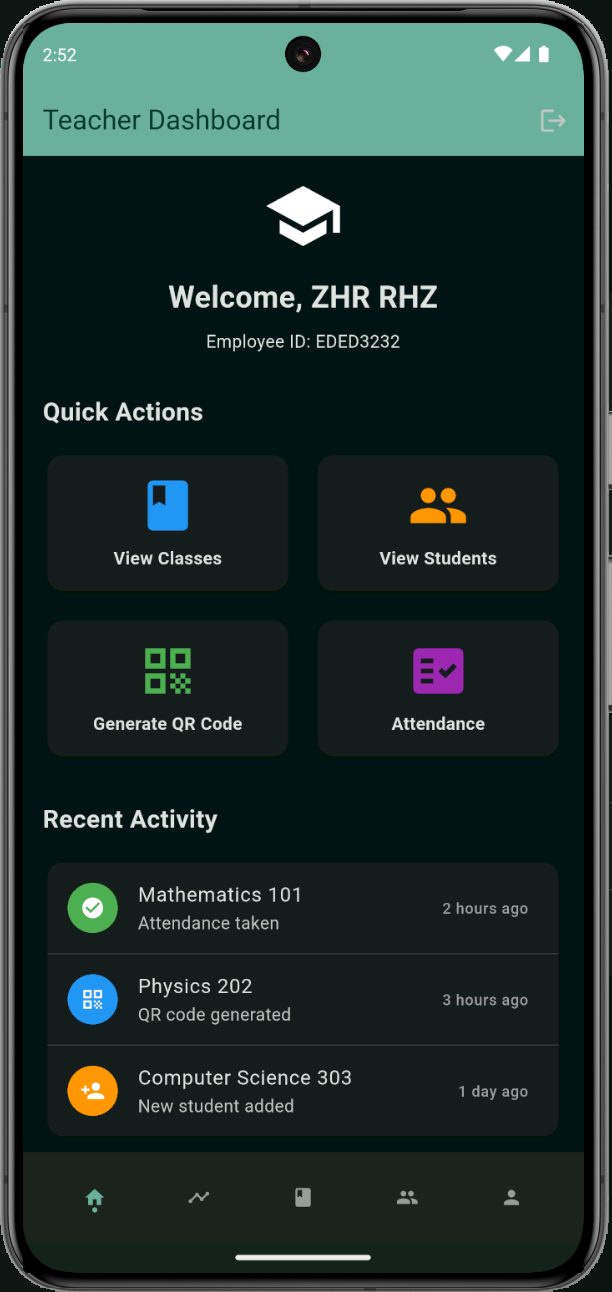
\includegraphics[width=\textwidth]{images/rachid/teacher-side-home.png}
        \caption{Mobile view showing quick access to key features and real-time attendance statistics}
    \end{subfigure}
    \hfill
    \begin{subfigure}[b]{0.48\textwidth}
        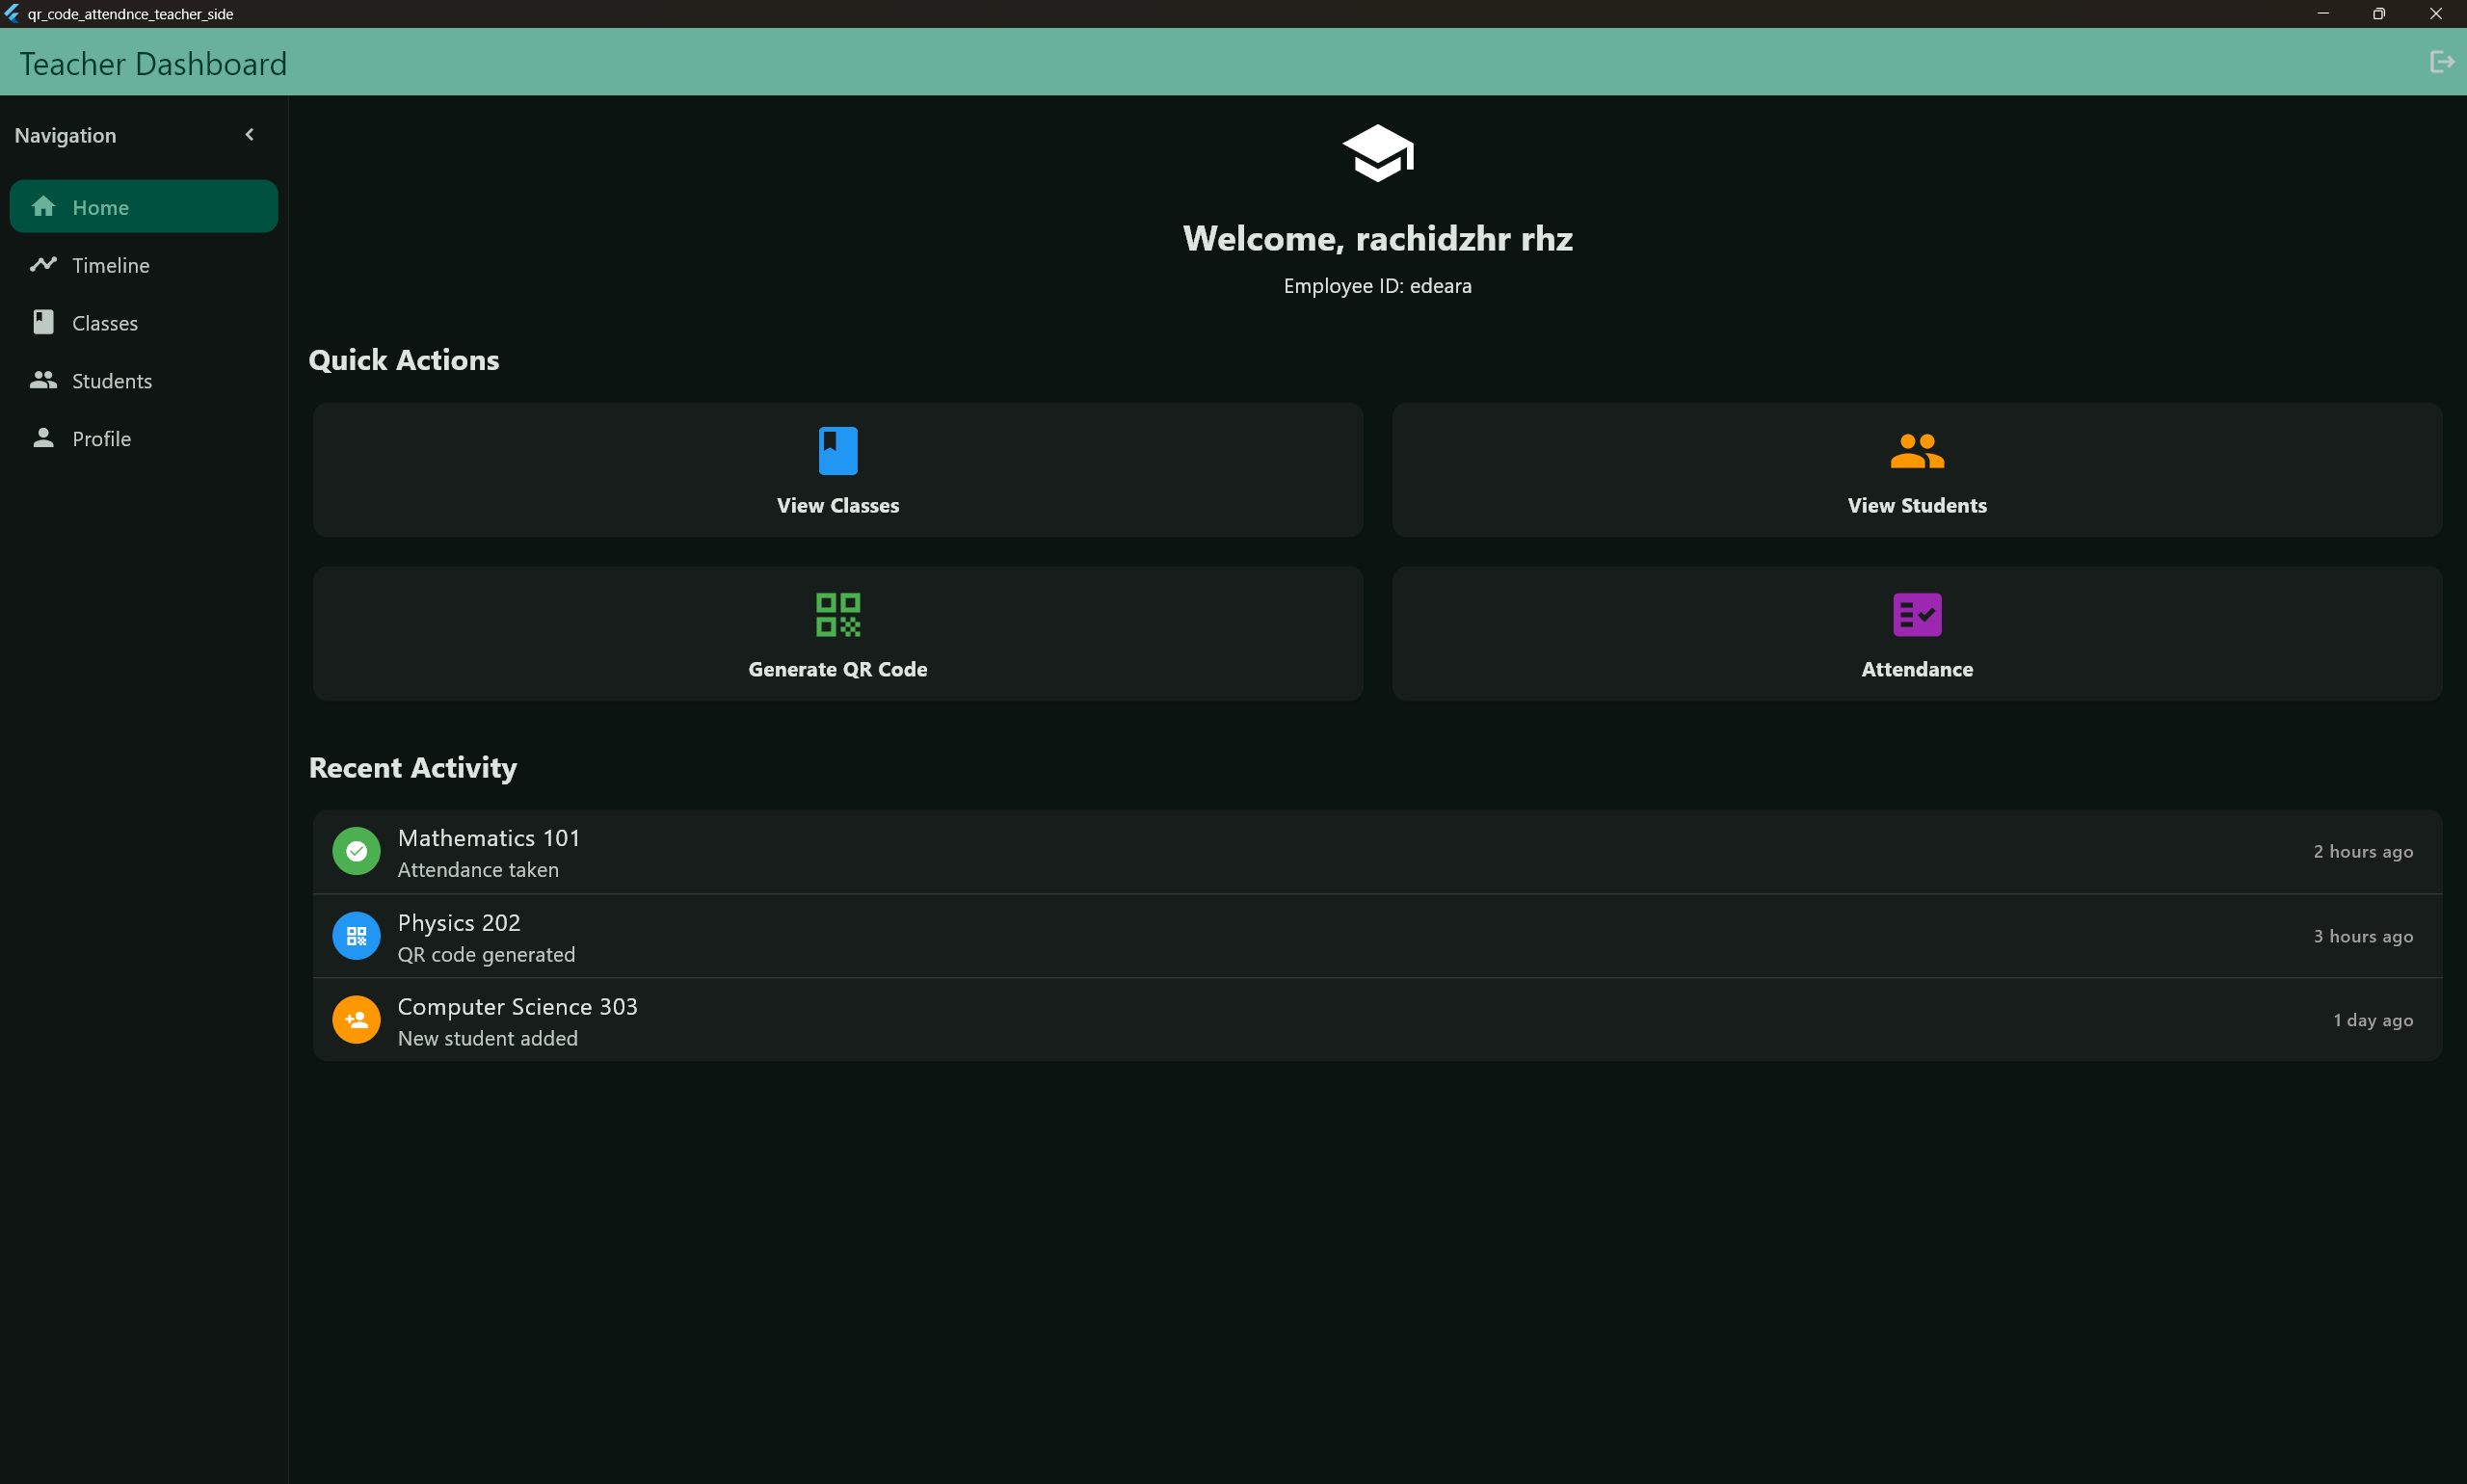
\includegraphics[width=\textwidth]{images/rachid/teacher-side-home-disktop.png}
        \caption{Desktop view with expanded navigation rail and detailed dashboard layout}
    \end{subfigure}
    \caption{Teacher's Home Dashboard Interface}
    \label{fig:home-interface}
\end{figure}

\paragraph{Profile Management}
\clearpage
\begin{figure}[H]
    \centering
    \begin{subfigure}[b]{0.48\textwidth}
        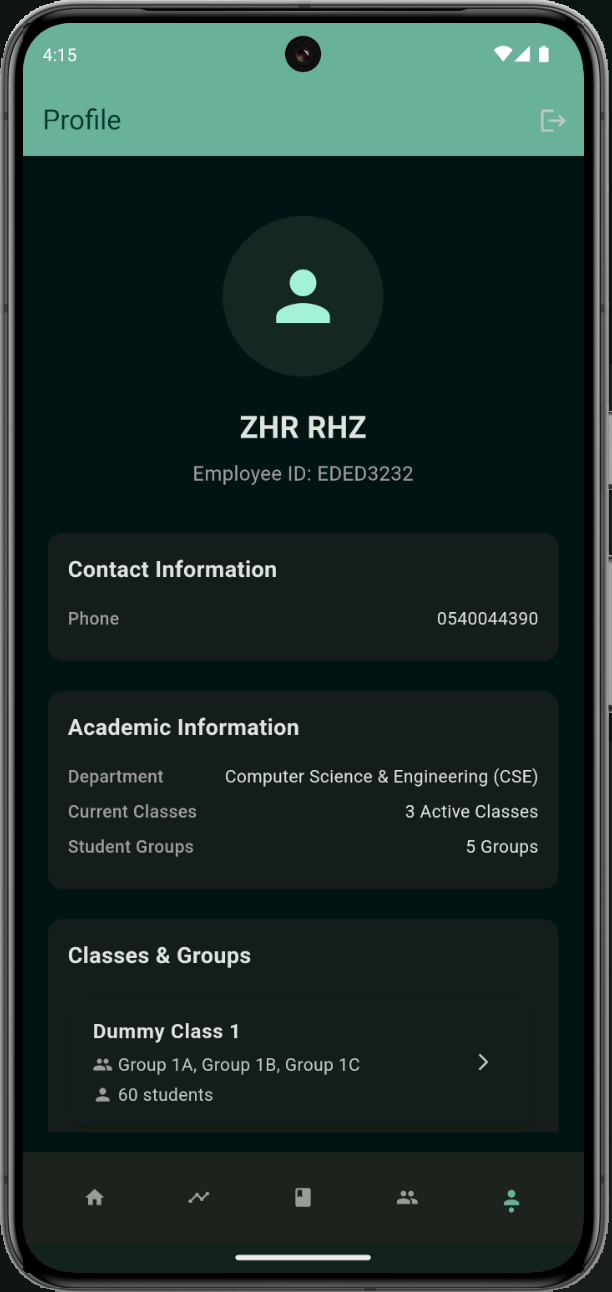
\includegraphics[width=\textwidth]{images/rachid/teacher-side-profile.png}
        \caption{Mobile view with compact profile information and quick actions}
    \end{subfigure}
    \hfill
    \begin{subfigure}[b]{0.48\textwidth}
        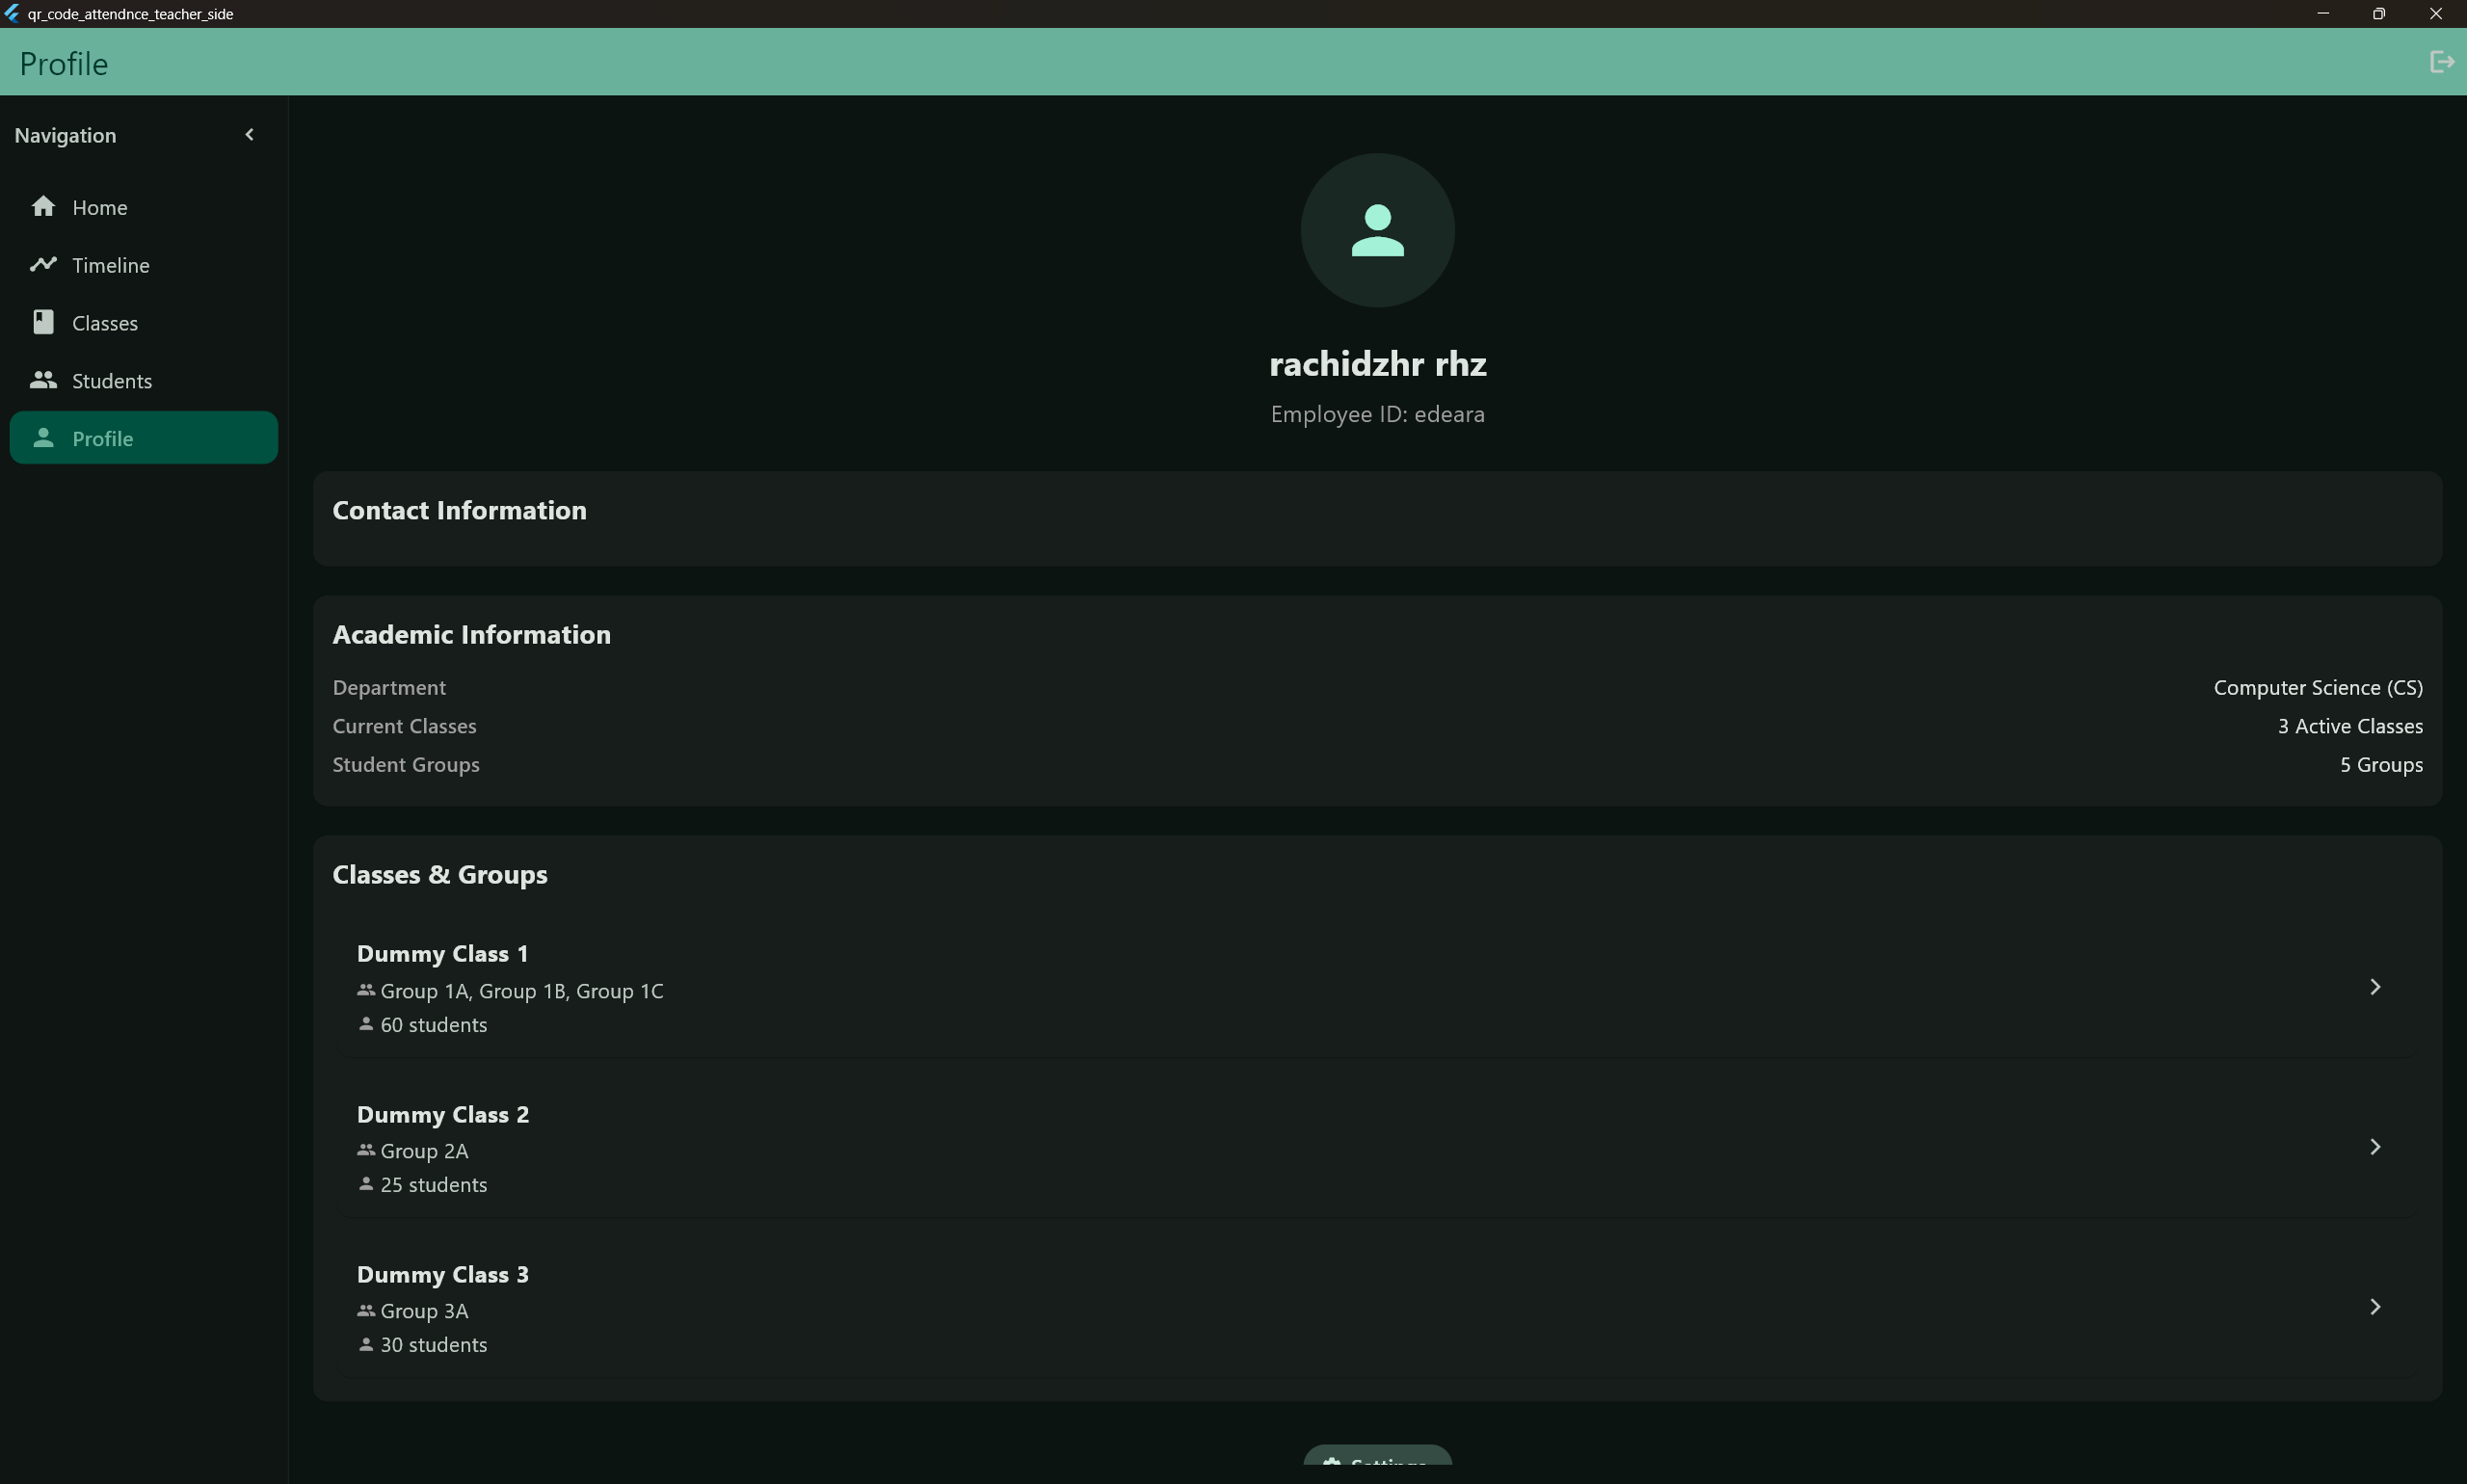
\includegraphics[width=\textwidth]{images/rachid/teacher-side-profile-disktop.png}
        \caption{Desktop view showing expanded profile details and statistics}
    \end{subfigure}
    \caption{Teacher Profile Management Interface}
    \label{fig:profile-interface}
\end{figure}

\paragraph{Settings Interface}
\vspace{1cm}
\begin{figure}[H]
    \centering
    \begin{subfigure}[b]{0.48\textwidth}
        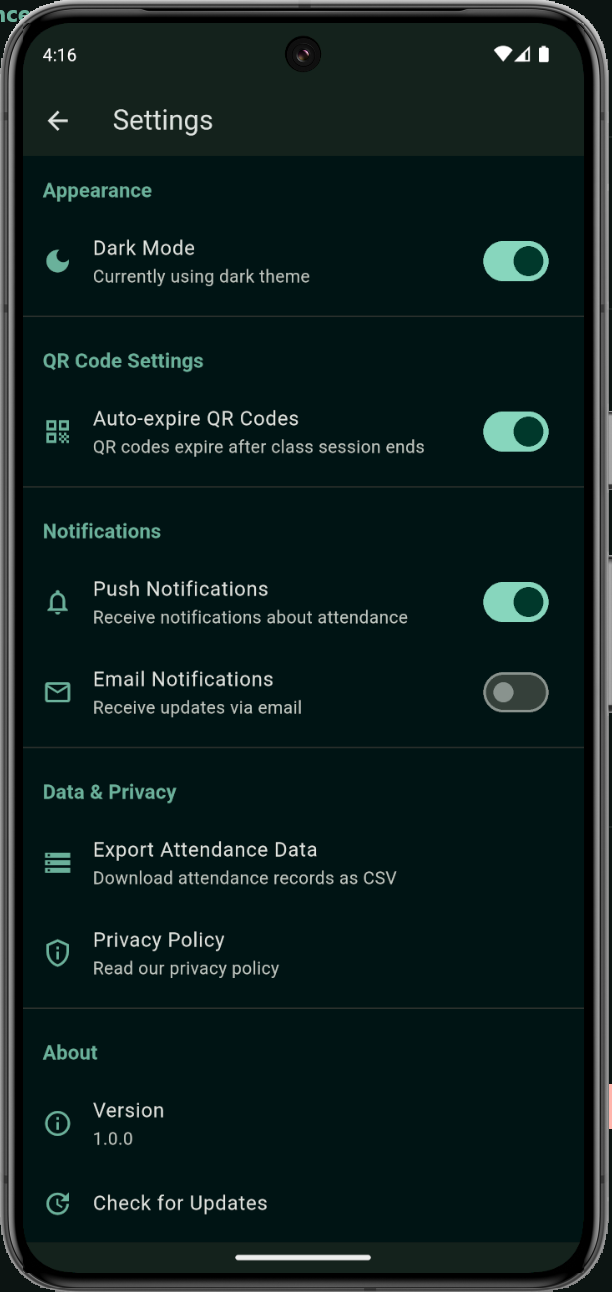
\includegraphics[width=\textwidth]{images/rachid/teacher-side-settings.png}
        \caption{Mobile settings view with scrollable preferences}
    \end{subfigure}
    \hfill
    \begin{subfigure}[b]{0.48\textwidth}
        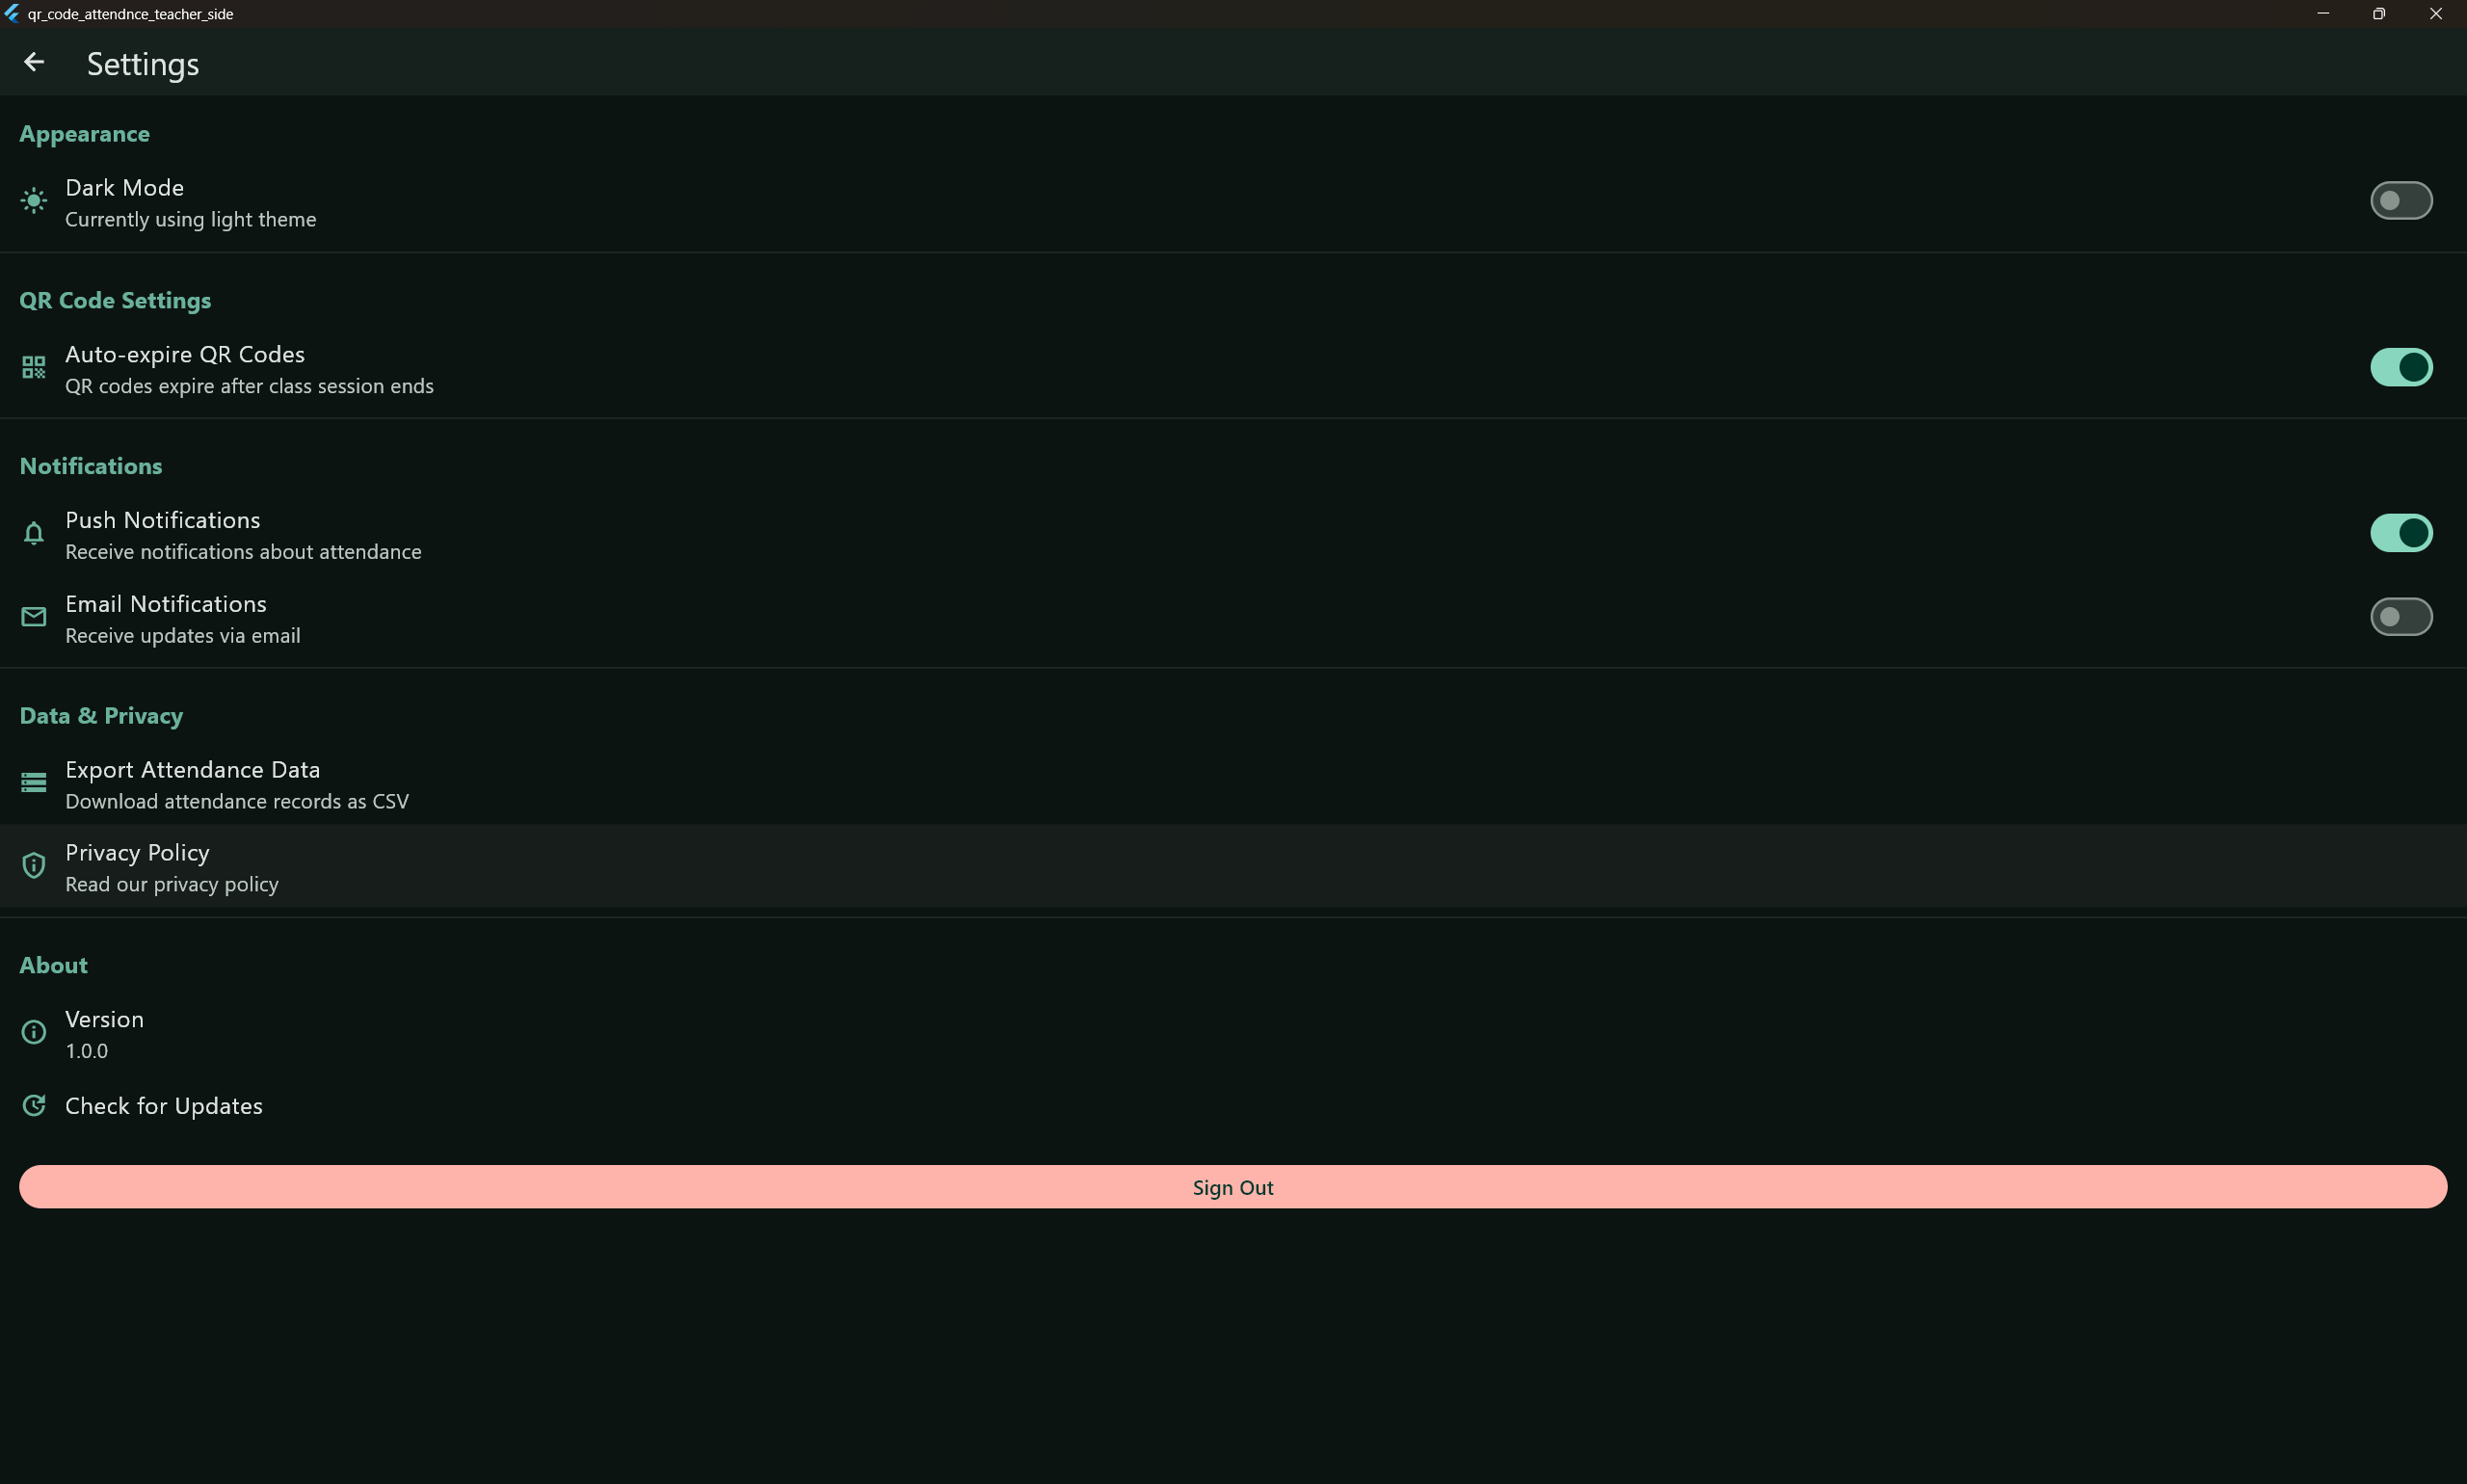
\includegraphics[width=\textwidth]{images/rachid/teacher-side-settings-desktop.png}
        \caption{Desktop settings panel with categorized options}
    \end{subfigure}
    \caption{Application Settings Interface}
    \label{fig:settings-interface}
\end{figure}

\paragraph{Student Management}
\vspace{1cm}
\begin{figure}[H]
    \centering
    \begin{subfigure}[b]{0.48\textwidth}
        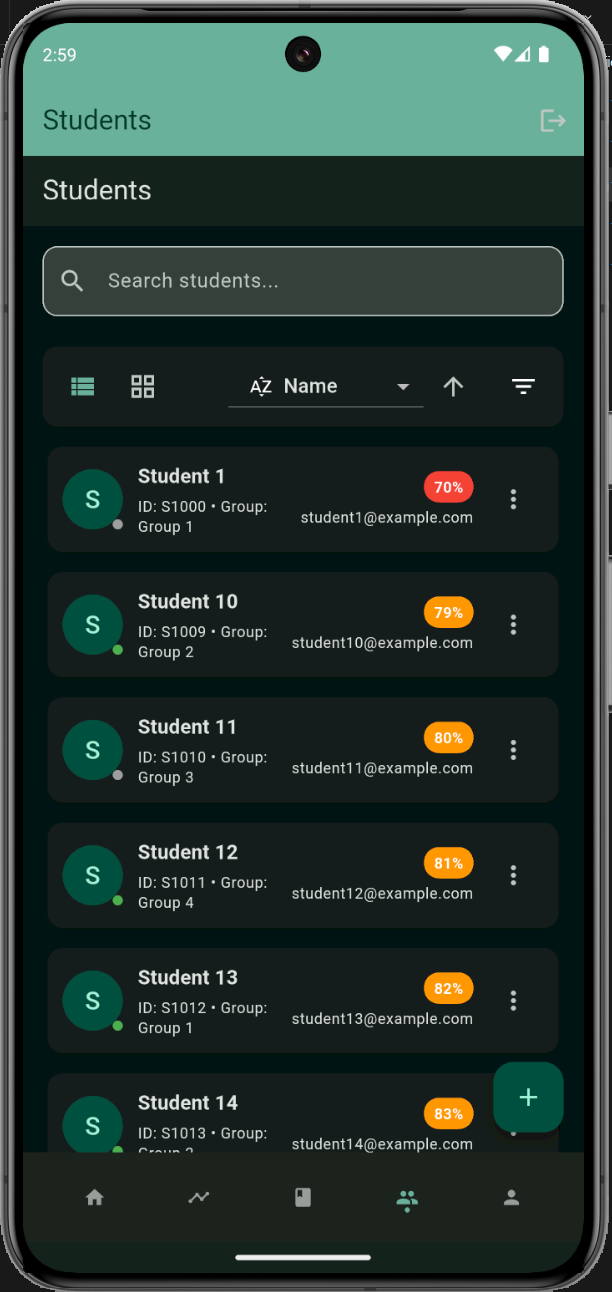
\includegraphics[width=\textwidth]{images/rachid/teacher-side-studentpage.png}
        \caption{Mobile student list with attendance status indicators}
    \end{subfigure}
    \hfill
    \begin{subfigure}[b]{0.48\textwidth}
        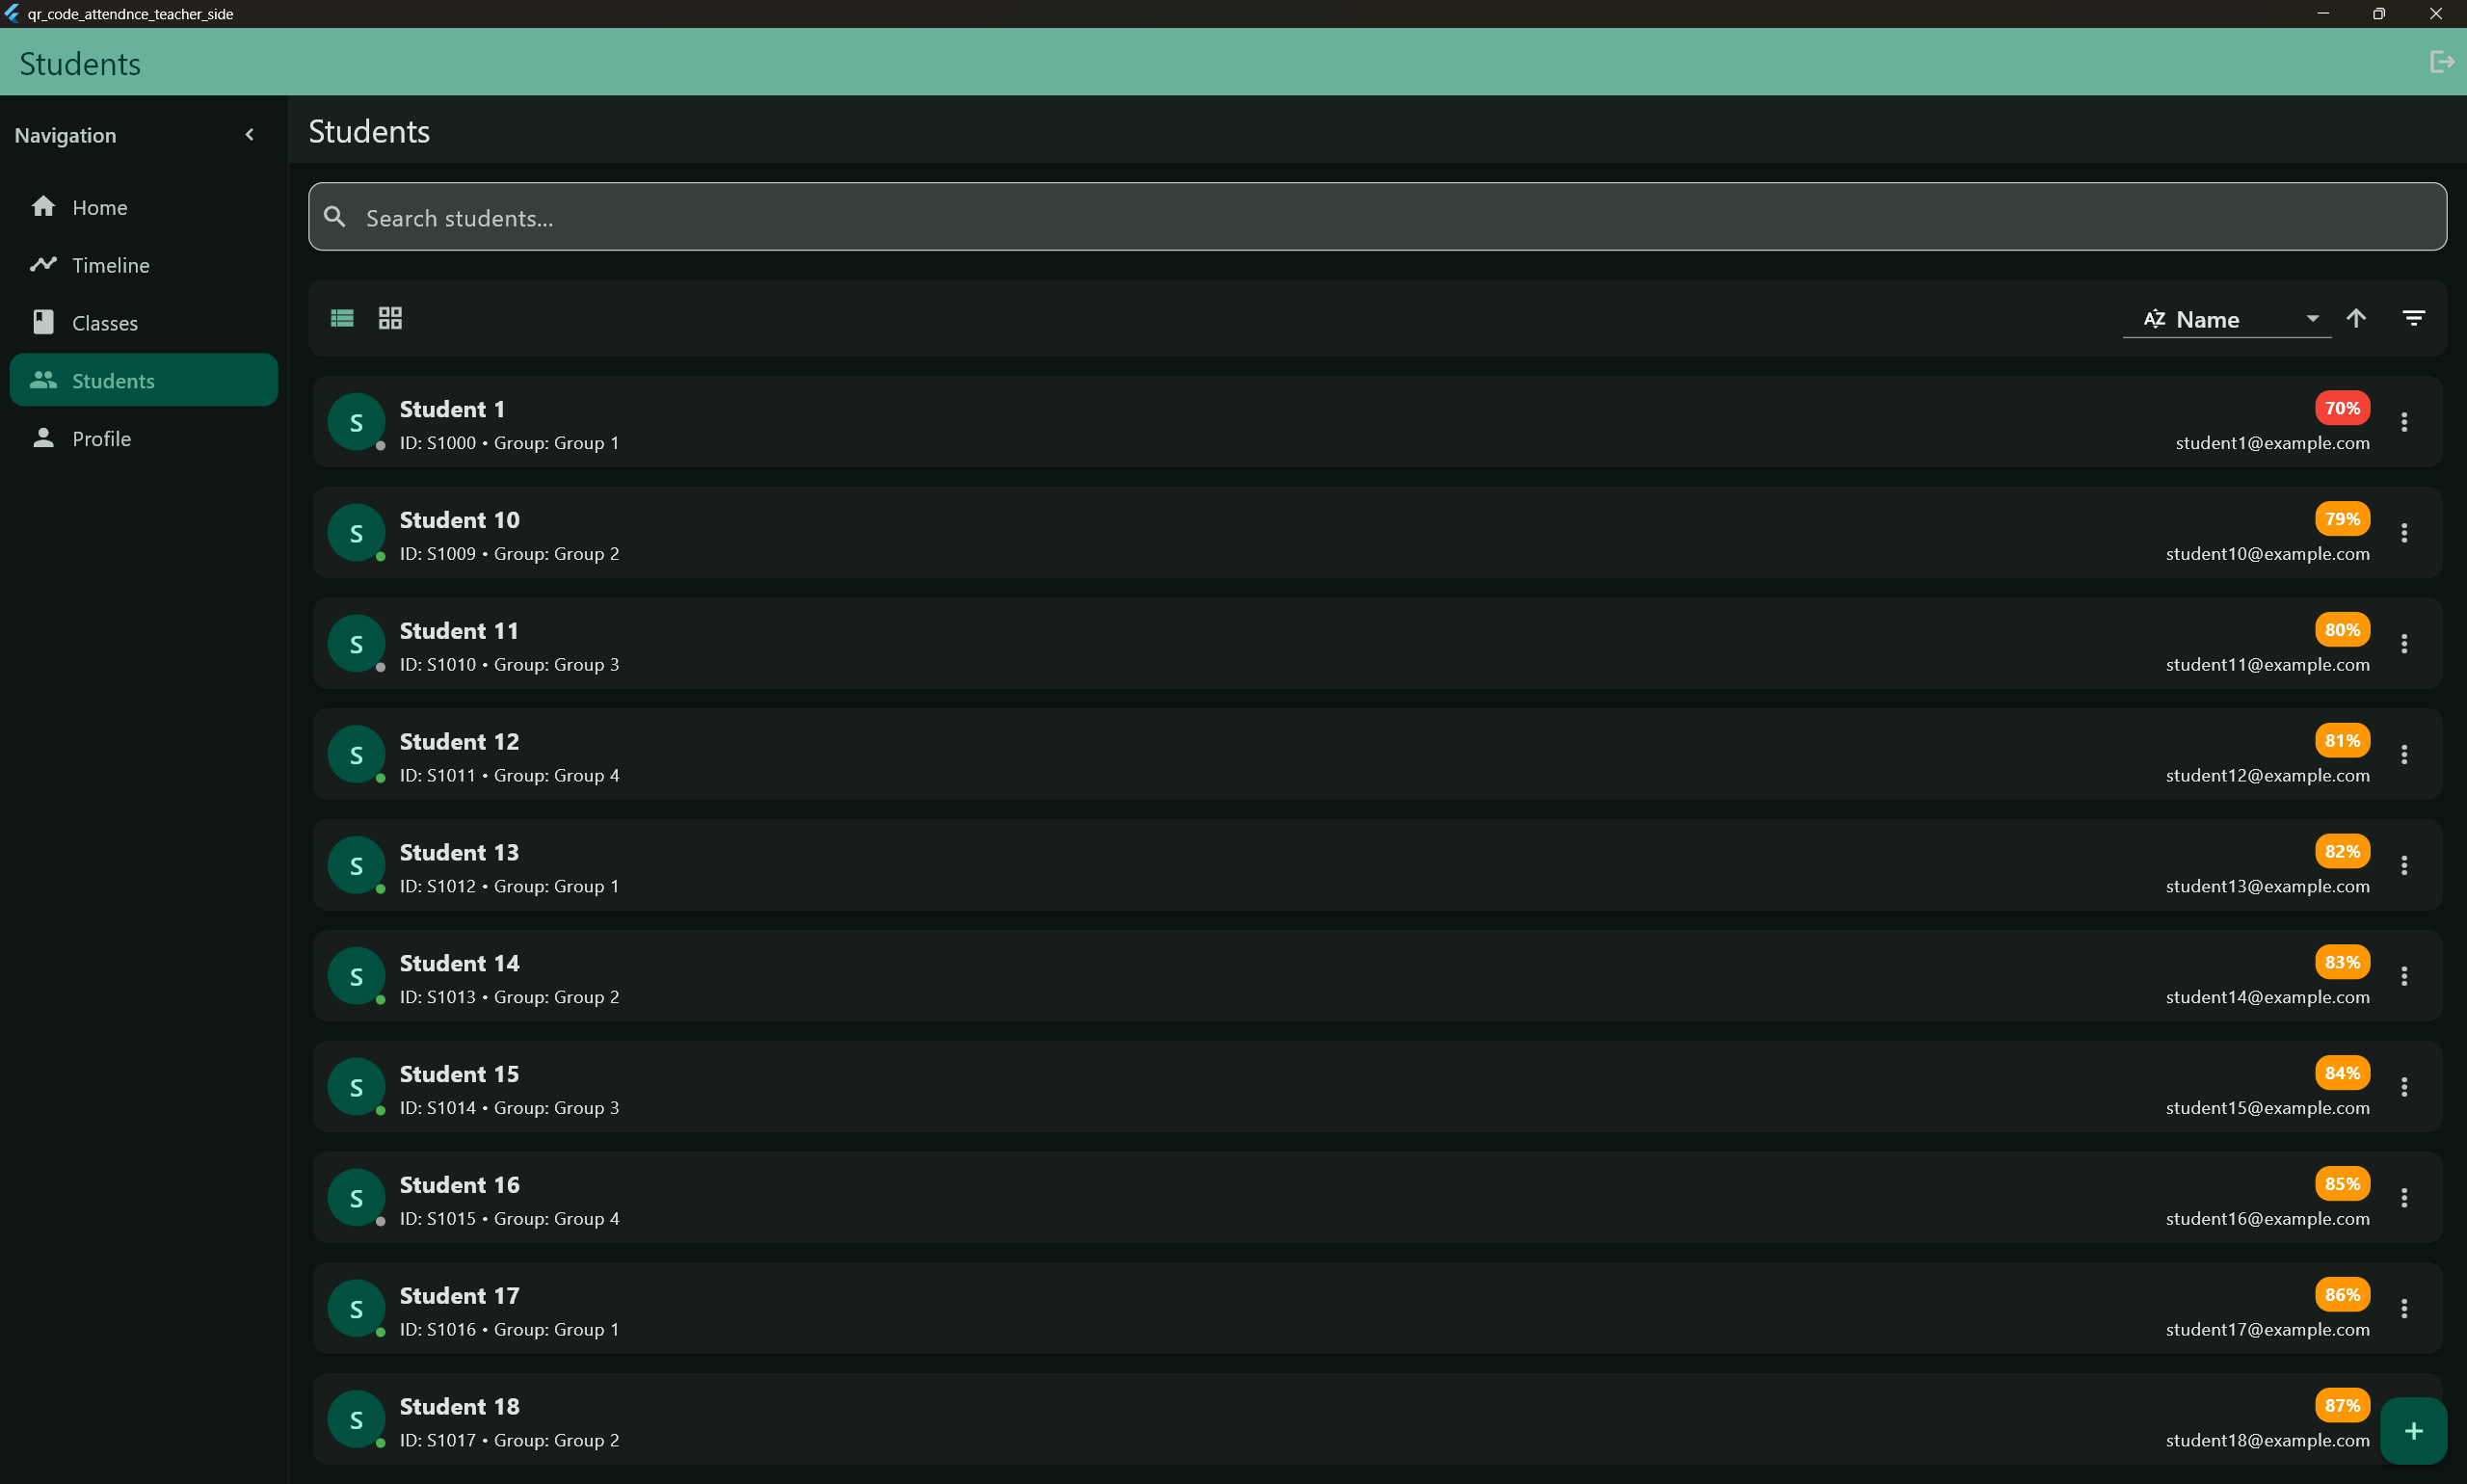
\includegraphics[width=\textwidth]{images/rachid/teacher-side-studentpage-desktop.png}
        \caption{Desktop view with enhanced student management tools}
    \end{subfigure}
    \caption{Student Management Interface}
    \label{fig:student-management}
\end{figure}

\paragraph{Student Profile View}
\vspace{1cm}
\begin{figure}[H]
    \centering
    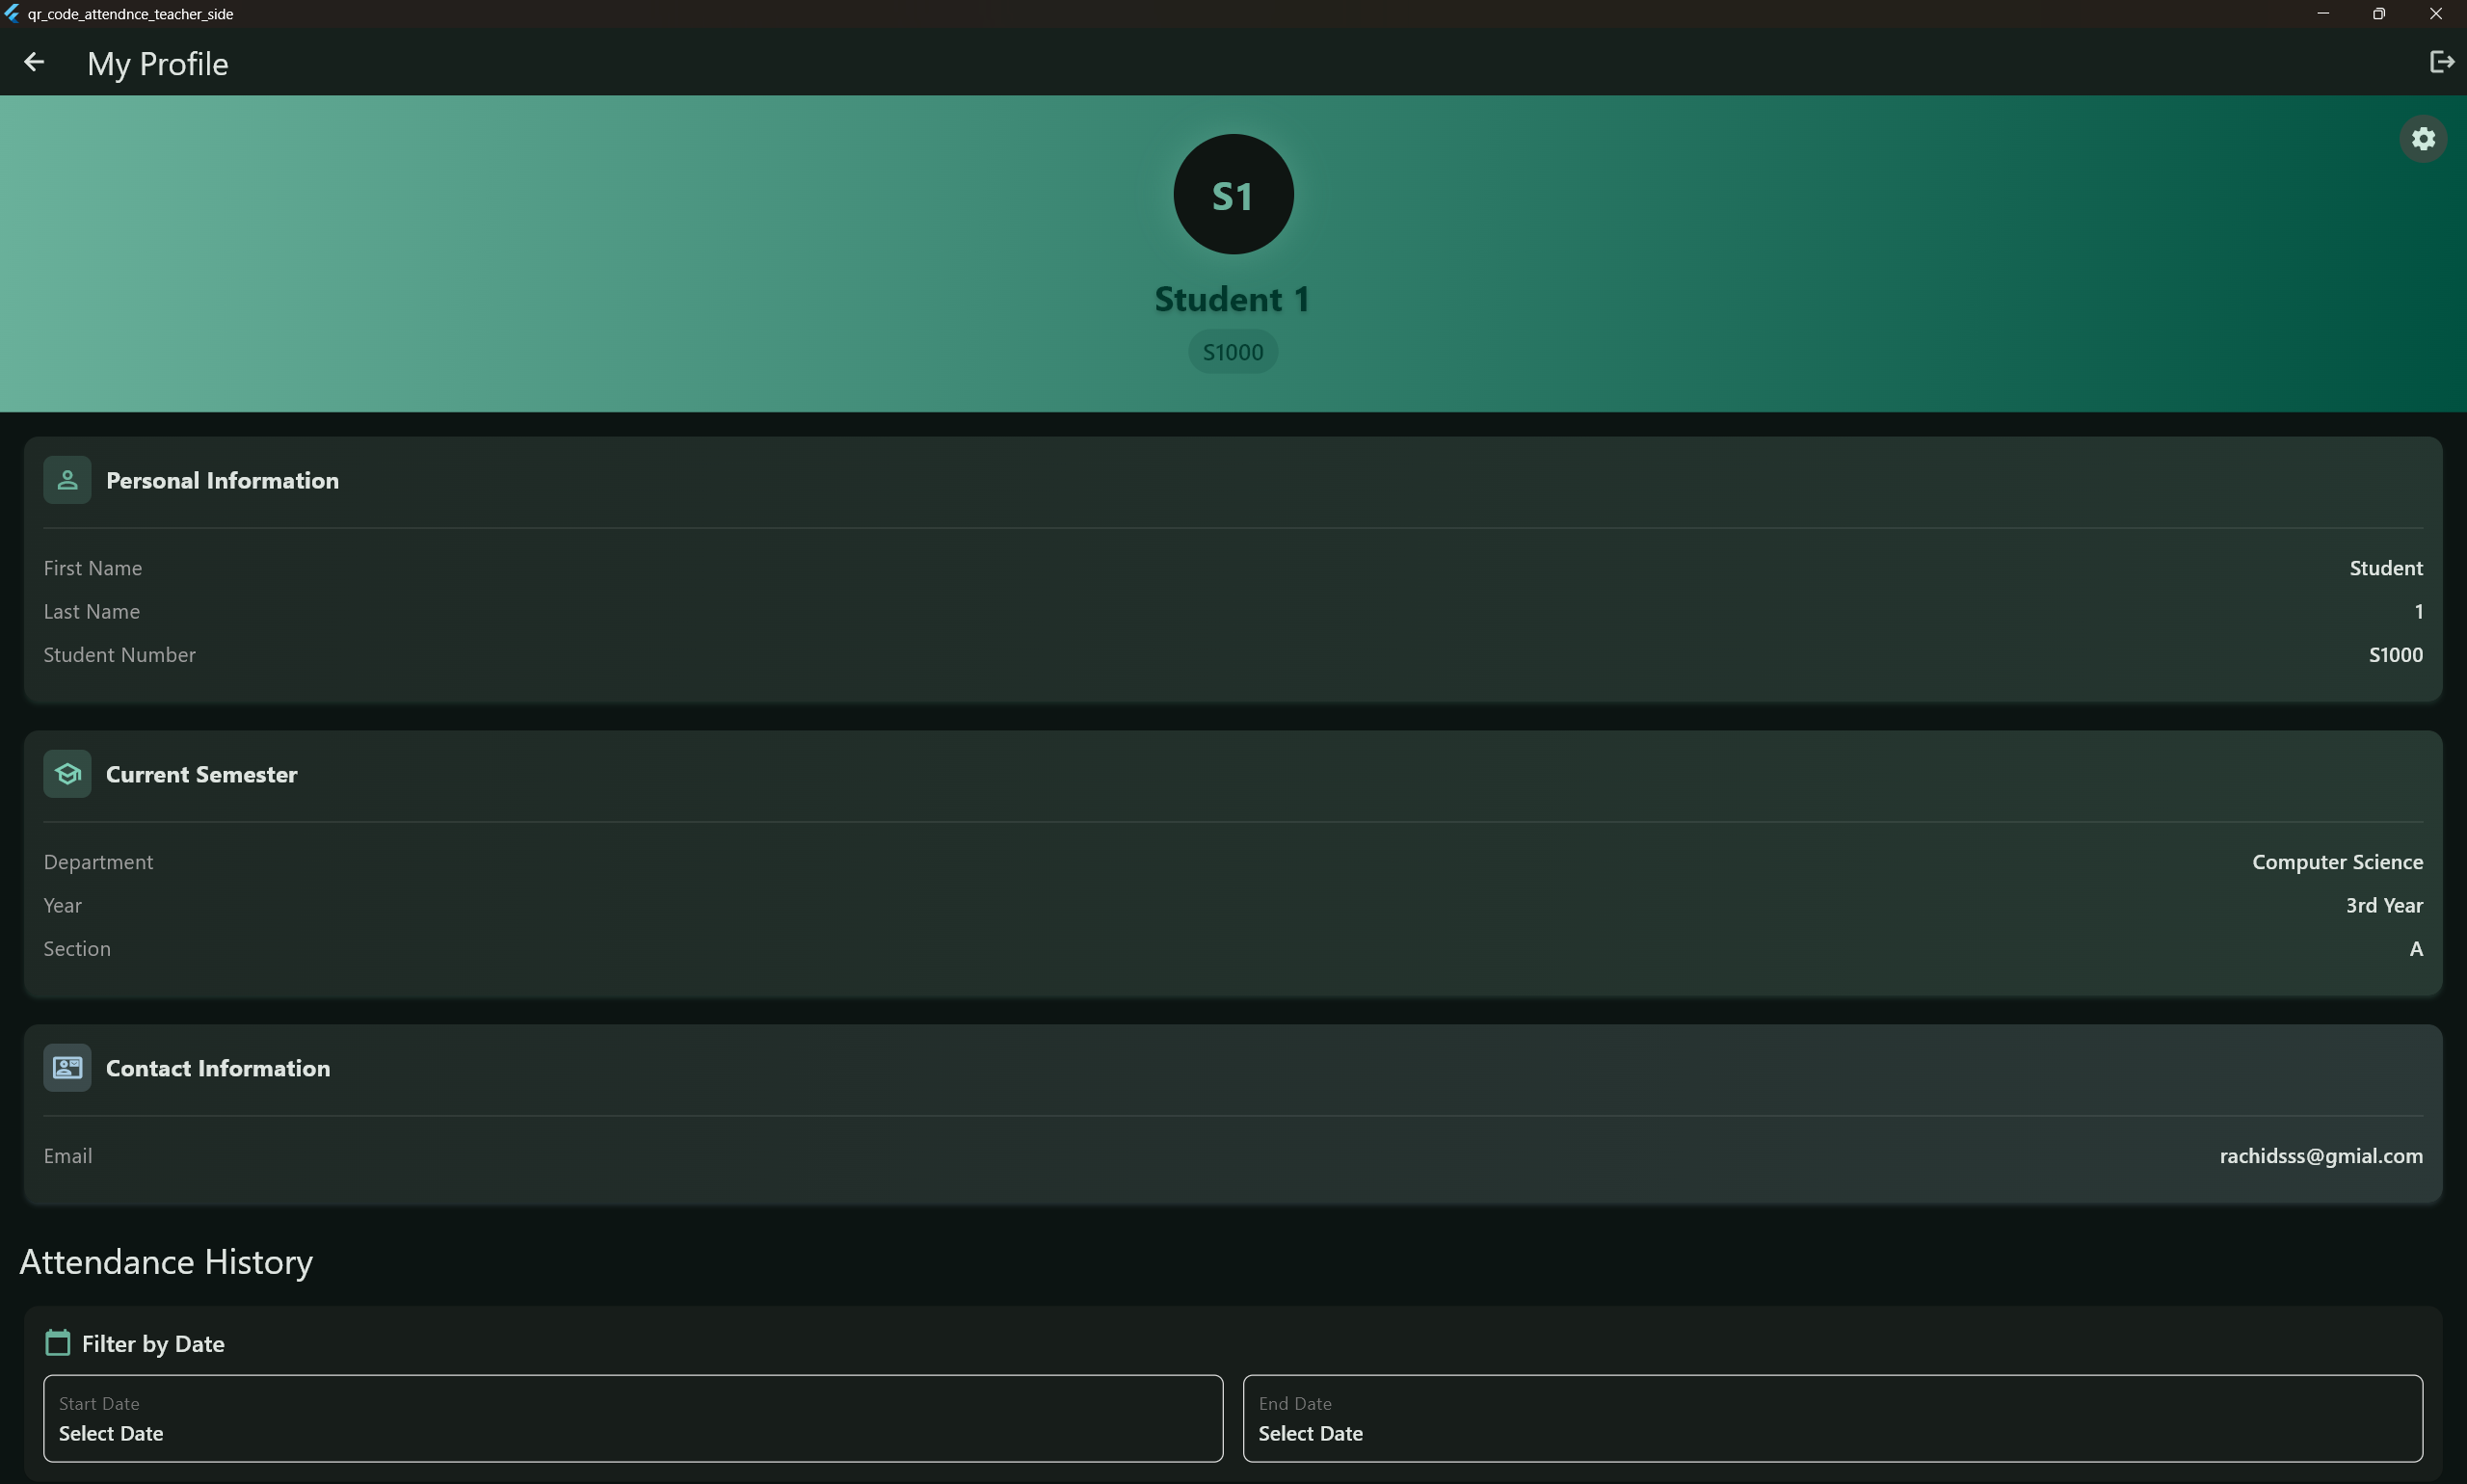
\includegraphics[width=0.8\textwidth]{images/rachid/teacher-side-studentpage-profileOfStudent-desktop.png}
    \caption{Detailed student profile view showing attendance history and academic information}
    \label{fig:student-profile}
\end{figure}

\paragraph{Attendance Timeline}
\vspace{1cm}
\begin{figure}[H]
    \centering
    \begin{subfigure}[b]{0.48\textwidth}
        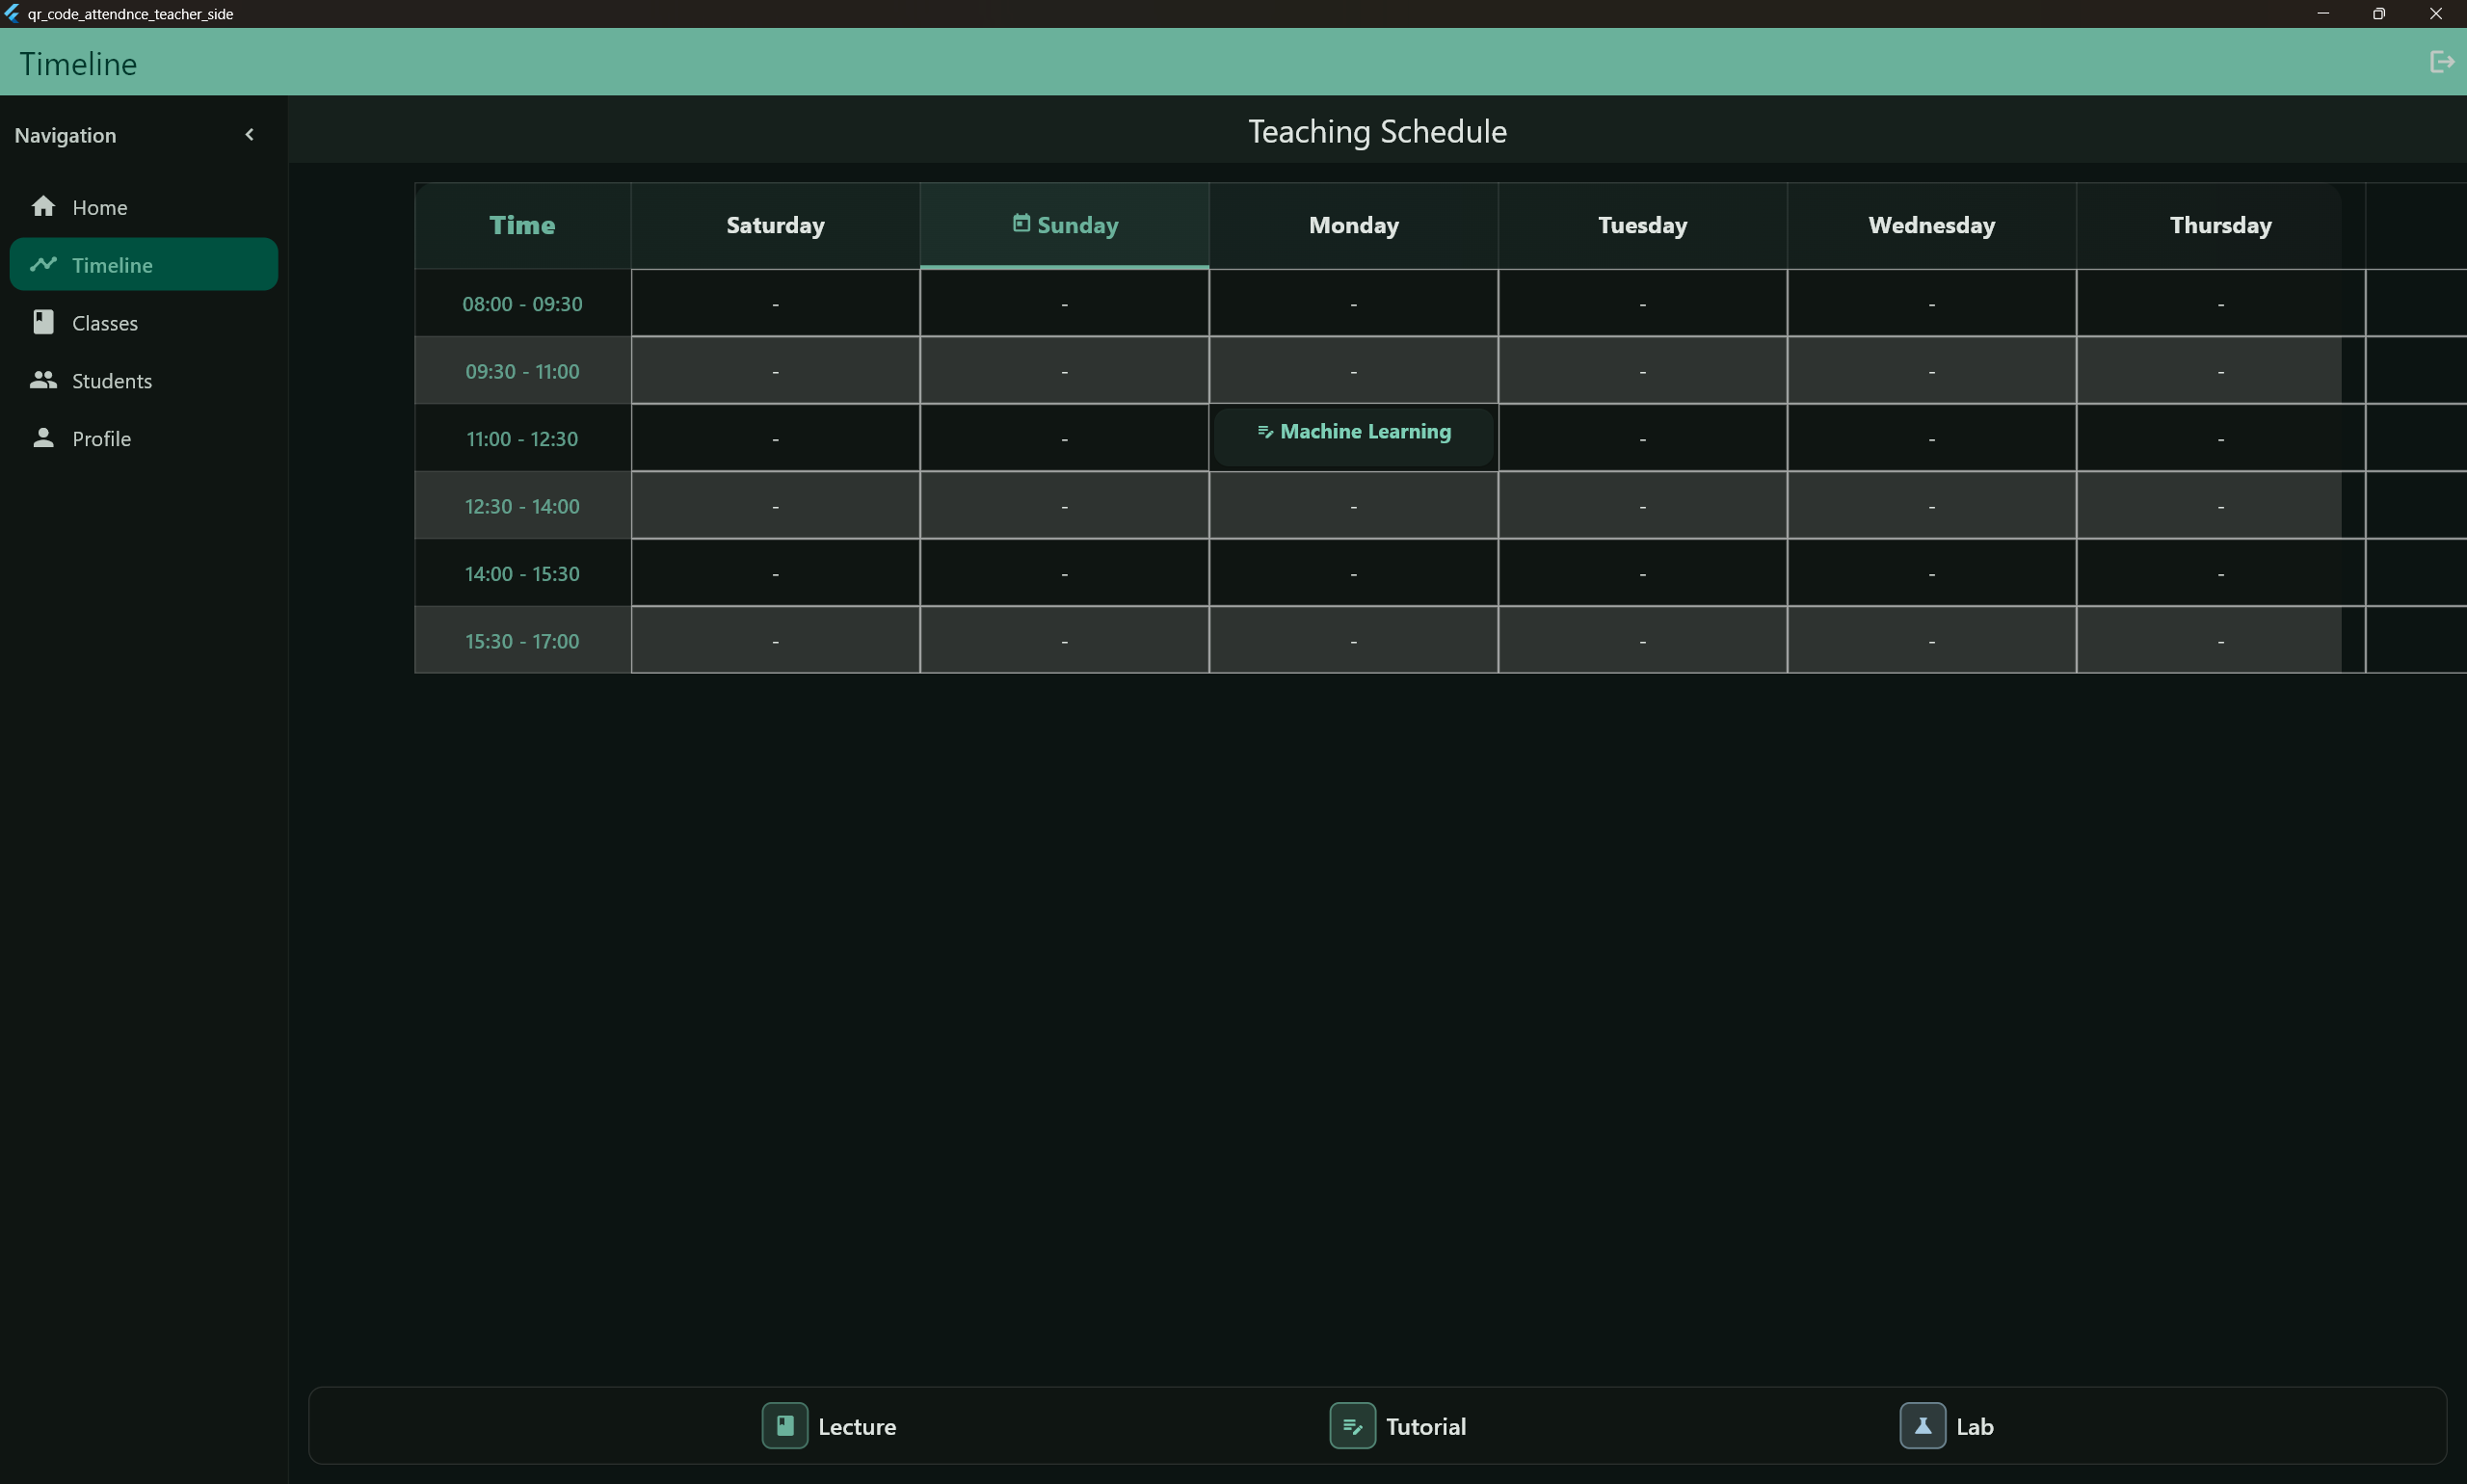
\includegraphics[width=\textwidth]{images/rachid/teacher-side-timeline.png}
        \caption{Mobile timeline view with chronological attendance events}
    \end{subfigure}
    \hfill
    \begin{subfigure}[b]{0.48\textwidth}
        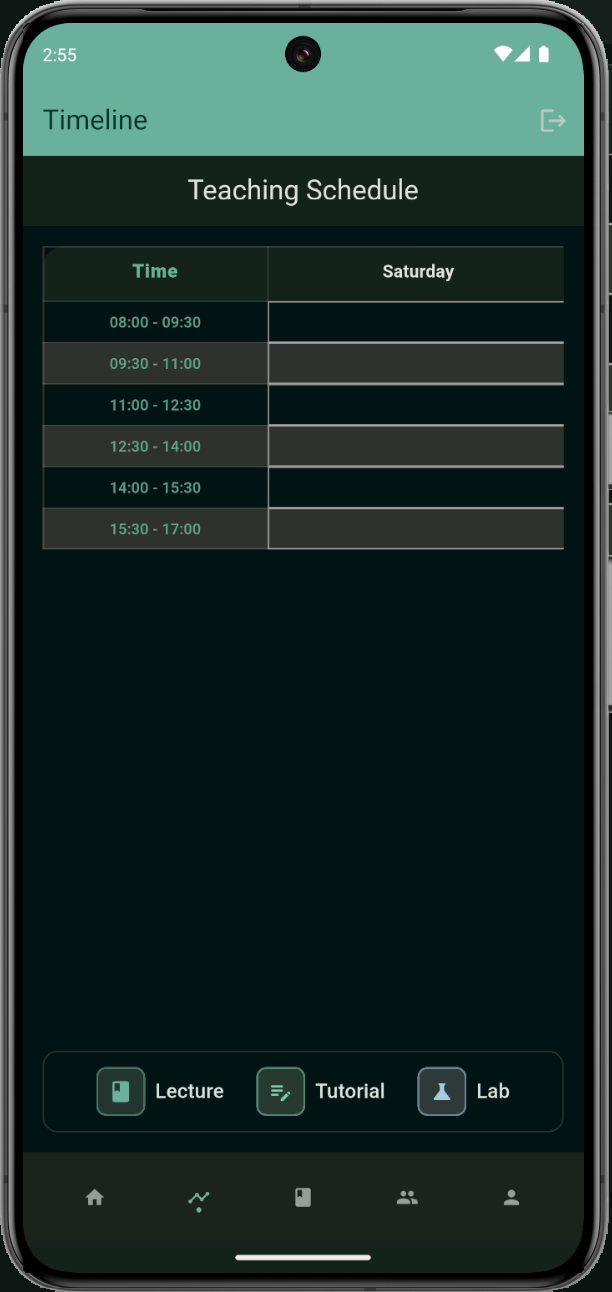
\includegraphics[width=\textwidth]{images/rachid/teacher-side-timeline-desktop.png}
        \caption{Desktop timeline with expanded event details and filtering options}
    \end{subfigure}
    \caption{Attendance Timeline Interface}
    \label{fig:timeline-interface}
\end{figure}








\newpage
\thispagestyle{empty}

\setcounter{chapter}{3}
\refstepcounter{chapter}

\phantomsection
\addcontentsline{toc}{chapter}{\protect\numberline{\thechapter}Conclusion}

\vspace*{\fill}
\begin{center}
    {\color{mintgreen} \rule{\textwidth}{2pt} }\\[0.5cm]
    {\Huge \textbf{Conclusion}}\\[0.5cm]
    {\color{mintgreen} \rule{0.8\textwidth}{1.5pt} }
\end{center}
\vspace*{\fill}
\begin{center}
    {\color{mintgreen} \rule{0.8\textwidth}{1.5pt} }\\[0.3cm]
    {\color{mintgreen} \rule{\textwidth}{2pt} }
\end{center}
\vspace{0.3cm}


\newpage
\begin{tcolorbox}[
    colback=mintgreen!20, 
    colframe=mintgreen!80!black, 
    width=\textwidth, 
    boxrule=1pt, 
    arc=5pt, 
    auto outer arc,
    left=10pt,
    right=10pt,
    top=6pt,
    bottom=6pt
]
    \centering
    \Large \textbf{Conclusion}
\end{tcolorbox}

\vspace{0.5cm} % Space between the box and the text

%\chapter*{} % Keep if you want it unnumbered; remove if already numbered elsewhere

This project was part of the digital transformation of the educational system through the design and development of a mobile application that enables student attendance tracking using QR code technology. The application addresses many of the shortcomings of traditional attendance methods, which are often inefficient, time-consuming, and prone to human error or fraud.

The developed application provides a reliable, fast, and secure solution for recording attendance by automating the process via QR code scanning and storing the data in a centralized, real-time database accessible by both teachers and administrators. This approach not only saves time but also promotes transparency and student accountability.

Among the key achievements of the project:
\begin{itemize}
  \item Implementation of an intuitive interface tailored to different user roles (teacher, student).
  \item Automatic recording of timestamped data to prevent manipulation.
  \item Integration of analytical tools to monitor attendance and absence patterns.
\end{itemize}

The potential applications of this solution extend beyond universities. It can be adapted to other educational or professional settings requiring rigorous attendance management.

However, the system has some limitations. It assumes that students have functioning smartphones and a stable internet connection when scanning the QR code. Moreover, relying solely on code scanning for authentication could be bypassed without additional verification mechanisms such as geolocation or biometric checks.

For future improvements, several directions can be considered:
\begin{itemize}
  \item Integration with Learning Management Systems (LMS) for a comprehensive student tracking ecosystem.
  \item Addition of geolocation to verify the student's physical presence in the classroom.
  \item Development of an advanced administrative dashboard for detailed attendance analytics.
\end{itemize}

In conclusion, this project marks a significant step toward intelligent and automated attendance management in educational institutions. It demonstrates our concrete contribution to enhancing academic processes by combining mobile technology, structured software modeling, and innovative educational practices.




% \chapter{Introduction}
\section{Project Overview}
\label{sec:overview}
This documentation describes a comprehensive QR code-based attendance tracking system implemented using Flutter and Supabase. The system consists of two main components: a teacher interface for managing attendance and generating QR codes, and a student interface for scanning QR codes to mark attendance.

\section{Objectives}
\begin{itemize}
    \item Streamline the attendance tracking process
    \item Reduce manual entry errors
    \item Provide real-time attendance statistics
    \item Enable efficient attendance management
\end{itemize}

\section{Navigation Guide}
\begin{itemize}
    \item \hyperref[sec:overview]{Project Overview}
    \item \hyperref[sec:tech_specs]{Technical Specifications}
    \item \hyperref[sec:architecture]{Application Architecture}
    \item \hyperref[sec:teacher_interface]{Teacher Interface Documentation}
    \item \hyperref[sec:student_interface]{Student Interface Documentation}
    \item \hyperref[sec:implementation]{Implementation Details}
    \item \hyperref[sec:practical]{Partie pratique}
\end{itemize}
% \section{Technical Specifications}
\label{sec:tech_specs}
\subsection{Hardware Requirements}
\begin{itemize}
    \item Mobile device with camera capability (for QR scanning)
    \item Internet connectivity
    \item Minimum device specifications:
    \begin{itemize}
        \item Android 6.0 or higher
        \item iOS 11.0 or higher
        \item 2GB RAM minimum
        \item Camera with autofocus
    \end{itemize}
\end{itemize}

\subsection{Software Stack}
\begin{itemize}
    \item Frontend: Flutter Framework
    \item Backend: Supabase
    \item Database: PostgreSQL
    \item Authentication: Supabase Auth
\end{itemize}

\subsection{Development Tools}
\begin{itemize}
    \item IDE: Visual Studio Code
    \item Version Control: Git
    \item State Management: Riverpod
    \item CI/CD: GitHub Actions
\end{itemize}

\section{Application Architecture}
\label{sec:architecture}
\subsection{System Architecture}
\begin{figure}[H]
    \centering
    \framebox{
        \begin{minipage}{0.8\textwidth}
            \centering
            \vspace{0.5cm}
            [System Architecture Diagram]\\
            \vspace{1cm}
            Place system architecture diagram here showing:\\
            \vspace{0.3cm}
            - Flutter Client\\
            - Supabase Backend\\
            - Database\\
            - Authentication Flow\\
            \vspace{0.5cm}
        \end{minipage}
    }
    \caption{System Architecture Diagram}
    \label{fig:system_architecture}
\end{figure}

\subsection{Database Schema}
\begin{figure}[H]
    \centering
    \framebox{
        \begin{minipage}{0.8\textwidth}
            \centering
            \vspace{0.5cm}
            [Database Schema Diagram]\\
            \vspace{1cm}
            Place database schema diagram here showing:\\
            \vspace{0.3cm}
            - User Tables\\
            - Attendance Tables\\
            - Course Tables\\
            - Relationships\\
            \vspace{0.5cm}
        \end{minipage}
    }
    \caption{Database Schema}
    \label{fig:database_schema}
\end{figure}
% \section{Implementation Details}
\label{sec:implementation}
\subsection{Core Features}
\begin{itemize}
    \item User authentication and authorization
    \item QR code generation and scanning
    \item Real-time attendance tracking
    \item Attendance report generation
    \item Profile management
\end{itemize}

\subsection{Implementation Challenges}
\begin{itemize}
    \item Handling offline scenarios
    \item QR code security measures
    \item Real-time synchronization
    \item Data consistency across devices
\end{itemize}

\subsection{Future Improvements}
\begin{itemize}
    \item Batch attendance processing
    \item Advanced analytics dashboard
    \item Integration with academic management systems
    \item Enhanced reporting features with export options
\end{itemize}
% \section{Teacher Interface Documentation}
\label{sec:teacher_interface}
\subsection{Overview}
The teacher interface provides comprehensive tools for managing attendance, generating QR codes, and monitoring student participation in real-time.

\subsection{Interface Components}
\subsubsection{Login Screen}
\begin{figure}[H]
    \centering
    \framebox{
        \begin{minipage}{0.8\textwidth}
            \centering
            \vspace{0.5cm}
            [Teacher Login Interface]\\
            \vspace{1cm}
            Screenshot of teacher login screen showing:\\
            \vspace{0.3cm}
            - Login Form\\
            - Authentication Options\\
            - Password Reset\\
            \vspace{0.5cm}
        \end{minipage}
    }
    \caption{Teacher Login Interface}
    \label{fig:teacher_login}
\end{figure}

\subsubsection{Dashboard}
\begin{figure}[H]
    \centering
    \framebox{
        \begin{minipage}{0.8\textwidth}
            \centering
            \vspace{0.5cm}
            [Teacher Dashboard]\\
            \vspace{1cm}
            Screenshot of teacher dashboard showing:\\
            \vspace{0.3cm}
            - Course List\\
            - Attendance Statistics\\
            - Quick Actions\\
            \vspace{0.5cm}
        \end{minipage}
    }
    \caption{Teacher Dashboard}
    \label{fig:teacher_dashboard}
\end{figure}

\subsubsection{QR Code Generation}
\begin{figure}[H]
    \centering
    \framebox{
        \begin{minipage}{0.8\textwidth}
            \centering
            \vspace{0.5cm}
            [QR Code Generation Interface]\\
            \vspace{1cm}
            Screenshot of QR generation screen showing:\\
            \vspace{0.3cm}
            - Course Selection\\
            - QR Code Display\\
            - Time Settings\\
            \vspace{0.5cm}
        \end{minipage}
    }
    \caption{QR Code Generation Interface}
    \label{fig:qr_generation}
\end{figure}

\subsubsection{Attendance Management}
\begin{figure}[H]
    \centering
    \framebox{
        \begin{minipage}{0.8\textwidth}
            \centering
            \vspace{0.5cm}
            [Attendance Management Interface]\\
            \vspace{1cm}
            Screenshot of attendance management showing:\\
            \vspace{0.3cm}
            - Student List\\
            - Attendance Records\\
            - Export Options\\
            \vspace{0.5cm}
        \end{minipage}
    }
    \caption{Attendance Management Interface}
    \label{fig:attendance_management}
\end{figure}

\subsubsection{Classes Screen}
The classes screen provides comprehensive class management functionality, allowing teachers to:
\begin{itemize}
    \item Create and manage course sections
    \item View enrolled students
    \item Access class-specific attendance records
    \item Manage course schedules
\end{itemize}

\subsubsection{Live Session Screen}
The live session screen enables real-time attendance monitoring with features including:
\begin{itemize}
    \item Active session management
    \item Real-time attendance updates
    \item Student participation tracking
    \item Session statistics
\end{itemize}

\subsubsection{Profile Screen}
The profile screen allows teachers to manage their personal and professional information:
\begin{itemize}
    \item Personal details
    \item Academic credentials
    \item Department affiliation
    \item Contact information
\end{itemize}

\subsubsection{Settings Screen}
The settings screen provides customization options:
\begin{itemize}
    \item Interface preferences
    \item Notification settings
    \item QR code generation defaults
    \item Privacy controls
\end{itemize}

\subsubsection{Teaching Schedule Screen}
The teaching schedule screen displays:
\begin{itemize}
    \item Weekly class timetable
    \item Course schedules
    \item Room assignments
    \item Schedule conflicts detection
\end{itemize}

\subsubsection{Students Screen}
The students screen provides a comprehensive view of:
\begin{itemize}
    \item Enrolled students by class
    \item Attendance statistics
    \item Student performance metrics
    \item Bulk actions for student management
\end{itemize}
% \section{Student Interface Documentation}
\label{sec:student_interface}
\subsection{Overview}
The student interface offers a streamlined experience for marking attendance through QR code scanning and viewing attendance history.

\subsection{Interface Components}
\subsubsection{Login Screen}
\begin{figure}[H]
    \centering
    \framebox{
        \begin{minipage}{0.8\textwidth}
            \centering
            \vspace{0.5cm}
            [Student Login Interface]\\
            \vspace{1cm}
            Screenshot of student login screen showing:\\
            \vspace{0.3cm}
            - Login Form\\
            - Student ID Entry\\
            - Password Reset\\
            \vspace{0.5cm}
        \end{minipage}
    }
    \caption{Student Login Interface}
    \label{fig:student_login}
\end{figure}

\subsubsection{QR Scanner}
\begin{figure}[H]
    \centering
    \framebox{
        \begin{minipage}{0.8\textwidth}
            \centering
            \vspace{0.5cm}
            [QR Scanner Interface]\\
            \vspace{1cm}
            Screenshot of QR scanner showing:\\
            \vspace{0.3cm}
            - Camera View\\
            - Scanning Guidelines\\
            - Success/Error Messages\\
            \vspace{0.5cm}
        \end{minipage}
    }
    \caption{QR Code Scanner Interface}
    \label{fig:qr_scanner}
\end{figure}

\subsubsection{Attendance History}
\begin{figure}[H]
    \centering
    \framebox{
        \begin{minipage}{0.8\textwidth}
            \centering
            \vspace{0.5cm}
            [Attendance History View]\\
            \vspace{1cm}
            Screenshot of attendance history showing:\\
            \vspace{0.3cm}
            - Course List\\
            - Attendance Dates\\
            - Statistics\\
            \vspace{0.5cm}
        \end{minipage}
    }
    \caption{Attendance History View}
    \label{fig:attendance_history}
\end{figure}

\subsubsection{Student Dashboard Screen}
The student dashboard provides a comprehensive overview of:
\begin{itemize}
    \item Current course enrollments
    \item Recent attendance records
    \item Upcoming classes
    \item Important notifications
\end{itemize}

\subsubsection{Student Courses Screen}
The courses screen displays detailed information about:
\begin{itemize}
    \item Enrolled courses
    \item Course schedules
    \item Attendance statistics per course
    \item Course materials and resources
\end{itemize}

\subsubsection{Student Profile Screen}
The profile screen allows students to manage:
\begin{itemize}
    \item Personal information
    \item Student ID details
    \item Contact information
    \item Academic profile
\end{itemize}

\subsubsection{Student Settings Screen}
The settings screen offers customization options for:
\begin{itemize}
    \item App preferences
    \item Notification settings
    \item Privacy controls
    \item Scanner configurations
\end{itemize}

\subsubsection{Student Timeline Screen}
The timeline screen provides a chronological view of:
\begin{itemize}
    \item Attendance history
    \item Class participation
    \item Important academic dates
    \item Schedule changes
\end{itemize}
% \section{Partie pratique}
\label{sec:practical}

\subsection{Implémentation de l'application}
L'implémentation de l'application a été réalisée en suivant une approche modulaire et structurée, en utilisant les meilleures pratiques de développement. Les principaux aspects de l'implémentation comprennent:

\subsubsection{Architecture du projet}
\begin{itemize}
    \item Structure MVC (Model-View-Controller)
    \item Organisation modulaire des fonctionnalités
    \item Séparation claire des responsabilités
    \item Gestion d'état avec Riverpod
\end{itemize}

\subsubsection{Fonctionnalités principales}
\begin{itemize}
    \item Système d'authentification sécurisé
    \item Génération et lecture de QR codes
    \item Suivi en temps réel des présences
    \item Interface adaptative (responsive design)
\end{itemize}

\subsubsection{Tests et assurance qualité}
\begin{itemize}
    \item Tests unitaires
    \item Tests d'intégration
    \item Tests de performance
    \item Revue de code systématique
\end{itemize}

\subsection{Caractéristiques des matériels utilisés}
Les caractéristiques matérielles minimales requises pour le bon fonctionnement de l'application sont:

\subsubsection{Configuration du serveur}
\begin{itemize}
    \item \textbf{Processeur:} Intel Xeon E5-2680 v4 ou équivalent
    \item \textbf{Mémoire RAM:} 16 GB DDR4
    \item \textbf{Stockage:} SSD 256 GB
    \item \textbf{Bande passante:} 100 Mbps minimum
\end{itemize}

\subsubsection{Configuration client (Desktop)}
\begin{itemize}
    \item \textbf{Processeur:} Intel Core i5 (8ème génération) ou équivalent
    \item \textbf{Mémoire RAM:} 8 GB minimum
    \item \textbf{Stockage:} 128 GB disponibles
    \item \textbf{Écran:} Résolution minimale de 1920x1080
\end{itemize}

\subsubsection{Configuration mobile}
\begin{itemize}
    \item \textbf{Processeur:} Snapdragon 665 ou équivalent
    \item \textbf{Mémoire RAM:} 4 GB minimum
    \item \textbf{Stockage:} 64 GB minimum
    \item \textbf{Caméra:} 8 MP minimum avec autofocus
\end{itemize}

\subsection{Caractéristiques des logiciels utilisés}
L'environnement logiciel nécessaire pour le développement et le déploiement de l'application comprend:

\subsubsection{Environnement de développement}
\begin{itemize}
    \item \textbf{Système d'exploitation:} Windows 10/11, macOS, Linux
    \item \textbf{IDE:} Visual Studio Code avec extensions Flutter/Dart
    \item \textbf{SDK:} Flutter 3.0 ou supérieur
    \item \textbf{Outils de versioning:} Git 2.30 ou supérieur
\end{itemize}

\subsubsection{Technologies utilisées}
\begin{itemize}
    \item \textbf{Framework:} Flutter
    \item \textbf{Language:} Dart 2.17 ou supérieur
    \item \textbf{Base de données:} PostgreSQL 13 ou supérieur
    \item \textbf{Backend:} Supabase
\end{itemize}

\subsubsection{Dépendances principales}
\begin{itemize}
    \item Flutter Riverpod pour la gestion d'état
    \item QR Flutter pour la génération de codes QR
    \item Mobile Scanner pour la lecture de codes QR
    \item Supabase Flutter SDK
\end{itemize}

\subsection{Présentation des interfaces}

\subsubsection{Interface desktop}
\begin{figure}[H]
    \centering
    \framebox{
        \begin{minipage}{0.8\textwidth}
            \centering
            \vspace{0.5cm}
            [Desktop Teacher Dashboard]\\
            \vspace{1cm}
            Screenshot montrant l'interface bureau avec:\\
            \vspace{0.3cm}
            - Navigation latérale\\
            - Liste des cours\\
            - Statistiques de présence\\
            - Génération de QR codes\\
            \vspace{0.5cm}
        \end{minipage}
    }
    \caption{Interface Bureau - Tableau de Bord Enseignant}
    \label{fig:desktop_teacher_dashboard}
\end{figure}

\subsubsection{Interface mobile}
\begin{figure}[H]
    \centering
    \framebox{
        \begin{minipage}{0.8\textwidth}
            \centering
            \vspace{0.5cm}
            [Mobile Teacher Interface]\\
            \vspace{1cm}
            Screenshot montrant l'interface mobile avec:\\
            \vspace{0.3cm}
            - Menu de navigation\\
            - Vue des présences\\
            - Contrôles QR code\\
            - Options rapides\\
            \vspace{0.5cm}
        \end{minipage}
    }
    \caption{Interface Mobile - Application Enseignant}
    \label{fig:mobile_teacher_interface}
\end{figure}



\begin{thebibliography}{9}
\bibitem{rayane2022}
Mehdi Rayane, Ladjeroud Khaoula, \textit{Une Application De Suivi De Présence Des étudiants Pour Les Enseignants}, Mémoire De Fin d'Etude, Université Mohammed Seddik Ben Yahia, Jijel, Algérie, 2022.

\bibitem{mekki2014}
Nacera Mekki, \textit{Réalisation d'un logiciel de gestion des absences pour les étudiants de l'E.P.S.T.T}, Mémoire de projet de fin d'études, Université Abou Bekr Belkaid, Tlemcen, Algérie, 2014.

\bibitem{omg2017}
Object Management Group, \textit{OMG Unified Modeling Language (UML), Version 2.5.1}, 2017.\\
Available: \url{https://www.omg.org/spec/UML/2.5.1/}

\bibitem{sommerville2015}
Ian Sommerville, \textit{Software Engineering}, 10th edition, Pearson, 2015.

\bibitem{pressman2014}
Roger S. Pressman, Bruce R. Maxim, \textit{Software Engineering: A Practitioner's Approach}, 8th Edition, McGraw-Hill, 2014.

\bibitem{royce1970}
Winston W. Royce, \textit{Managing the Development of Large Software Systems}, Proceedings of IEEE WESCON, pp. 1-9, 1970.

\bibitem{boehm1988}
Barry W. Boehm, \textit{A Spiral Model of Software Development and Enhancement}, Computer, vol. 21, no. 5, pp. 61-72, 1988.

\bibitem{beck2001}
Kent Beck et al., \textit{Manifesto for Agile Software Development}, 2001.\\
Available: \url{http://agilemanifesto.org}

\bibitem{cockburn2002}
Alistair Cockburn, \textit{Agile Software Development}, Addison-Wesley, 2002.

\bibitem{booch1994}
Grady Booch, \textit{Object-Oriented Analysis and Design with Applications}, 2nd Edition, Benjamin/Cummings Publishing, 1994.

\bibitem{gamma1995}
Erich Gamma, Richard Helm, Ralph Johnson, John Vlissides, \textit{Design Patterns: Elements of Reusable Object-Oriented Software}, Addison-Wesley, 1995.

\bibitem{rumbaugh2004}
James Rumbaugh, Ivar Jacobson, Grady Booch, \textit{The Unified Modeling Language Reference Manual}, 2nd Edition, Addison-Wesley, 2004.


\bibitem{fowler2004}
Martin Fowler, \textit{UML Distilled: A Brief Guide to the Standard Object Modeling Language}, 3rd Edition, Addison-Wesley, 2004.

\bibitem{bruegge2010}
Bernd Bruegge, Allen H. Dutoit, \textit{Object-Oriented Software Engineering Using UML, Patterns, and Java}, Prentice Hall, 2010.

\bibitem{arlow2005}
Jim Arlow, Ila Neustadt, \textit{UML 2 and the Unified Process}, 2nd Edition, Addison-Wesley, 2005.

\bibitem{booch2005uml}
Grady Booch, James Rumbaugh, Ivar Jacobson, \textit{The Unified Modeling Language User Guide}, Addison-Wesley, 2005.

\end{thebibliography}

\end{document}

